\documentclass[twoside]{book}

% Packages required by doxygen
\usepackage{fixltx2e}
\usepackage{calc}
\usepackage{doxygen}
\usepackage[export]{adjustbox} % also loads graphicx
\usepackage{graphicx}
\usepackage[utf8]{inputenc}
\usepackage{makeidx}
\usepackage{multicol}
\usepackage{multirow}
\PassOptionsToPackage{warn}{textcomp}
\usepackage{textcomp}
\usepackage[nointegrals]{wasysym}
\usepackage[table]{xcolor}

% Font selection
\usepackage[T1]{fontenc}
\usepackage[scaled=.90]{helvet}
\usepackage{courier}
\usepackage{amssymb}
\usepackage{sectsty}
\renewcommand{\familydefault}{\sfdefault}
\allsectionsfont{%
  \fontseries{bc}\selectfont%
  \color{darkgray}%
}
\renewcommand{\DoxyLabelFont}{%
  \fontseries{bc}\selectfont%
  \color{darkgray}%
}
\newcommand{\+}{\discretionary{\mbox{\scriptsize$\hookleftarrow$}}{}{}}

% Page & text layout
\usepackage{geometry}
\geometry{%
  a4paper,%
  top=2.5cm,%
  bottom=2.5cm,%
  left=2.5cm,%
  right=2.5cm%
}
\tolerance=750
\hfuzz=15pt
\hbadness=750
\setlength{\emergencystretch}{15pt}
\setlength{\parindent}{0cm}
\setlength{\parskip}{3ex plus 2ex minus 2ex}
\makeatletter
\renewcommand{\paragraph}{%
  \@startsection{paragraph}{4}{0ex}{-1.0ex}{1.0ex}{%
    \normalfont\normalsize\bfseries\SS@parafont%
  }%
}
\renewcommand{\subparagraph}{%
  \@startsection{subparagraph}{5}{0ex}{-1.0ex}{1.0ex}{%
    \normalfont\normalsize\bfseries\SS@subparafont%
  }%
}
\makeatother

% Headers & footers
\usepackage{fancyhdr}
\pagestyle{fancyplain}
\fancyhead[LE]{\fancyplain{}{\bfseries\thepage}}
\fancyhead[CE]{\fancyplain{}{}}
\fancyhead[RE]{\fancyplain{}{\bfseries\leftmark}}
\fancyhead[LO]{\fancyplain{}{\bfseries\rightmark}}
\fancyhead[CO]{\fancyplain{}{}}
\fancyhead[RO]{\fancyplain{}{\bfseries\thepage}}
\fancyfoot[LE]{\fancyplain{}{}}
\fancyfoot[CE]{\fancyplain{}{}}
\fancyfoot[RE]{\fancyplain{}{\bfseries\scriptsize Generated by Doxygen }}
\fancyfoot[LO]{\fancyplain{}{\bfseries\scriptsize Generated by Doxygen }}
\fancyfoot[CO]{\fancyplain{}{}}
\fancyfoot[RO]{\fancyplain{}{}}
\renewcommand{\footrulewidth}{0.4pt}
\renewcommand{\chaptermark}[1]{%
  \markboth{#1}{}%
}
\renewcommand{\sectionmark}[1]{%
  \markright{\thesection\ #1}%
}

% Indices & bibliography
\usepackage{natbib}
\usepackage[titles]{tocloft}
\setcounter{tocdepth}{3}
\setcounter{secnumdepth}{5}
\makeindex

% Hyperlinks (required, but should be loaded last)
\usepackage{ifpdf}
\ifpdf
  \usepackage[pdftex,pagebackref=true]{hyperref}
\else
  \usepackage[ps2pdf,pagebackref=true]{hyperref}
\fi
\hypersetup{%
  colorlinks=true,%
  linkcolor=blue,%
  citecolor=blue,%
  unicode%
}

% Custom commands
\newcommand{\clearemptydoublepage}{%
  \newpage{\pagestyle{empty}\cleardoublepage}%
}

\usepackage{caption}
\captionsetup{labelsep=space,justification=centering,font={bf},singlelinecheck=off,skip=4pt,position=top}

%===== C O N T E N T S =====

\begin{document}

% Titlepage & ToC
\hypersetup{pageanchor=false,
             bookmarksnumbered=true,
             pdfencoding=unicode
            }
\pagenumbering{alph}
\begin{titlepage}
\vspace*{7cm}
\begin{center}%
{\Large Ultrasonic distance measurer }\\
\vspace*{1cm}
{\large Generated by Doxygen 1.8.12}\\
\end{center}
\end{titlepage}
\clearemptydoublepage
\pagenumbering{roman}
\tableofcontents
\clearemptydoublepage
\pagenumbering{arabic}
\hypersetup{pageanchor=true}

%--- Begin generated contents ---
\chapter{File Index}
\section{File List}
Here is a list of all documented files with brief descriptions\+:\begin{DoxyCompactList}
\item\contentsline{section}{S\+R\+C/\+H\+W/{\bfseries button.\+h} }{\pageref{button_8h}}{}
\item\contentsline{section}{S\+R\+C/\+H\+W/{\bfseries gpio.\+h} }{\pageref{gpio_8h}}{}
\item\contentsline{section}{S\+R\+C/\+H\+W/{\bfseries lcd.\+h} }{\pageref{lcd_8h}}{}
\item\contentsline{section}{S\+R\+C/\+H\+W/\hyperlink{ultra_s_8h}{ultra\+S.\+h} \\*Header file for the ultrasonic module }{\pageref{ultra_s_8h}}{}
\item\contentsline{section}{S\+R\+C/\+M\+C\+U/{\bfseries application.\+h} }{\pageref{application_8h}}{}
\item\contentsline{section}{S\+R\+C/\+M\+C\+U/{\bfseries clock.\+h} }{\pageref{clock_8h}}{}
\item\contentsline{section}{S\+R\+C/\+M\+C\+U/{\bfseries counter.\+h} }{\pageref{counter_8h}}{}
\item\contentsline{section}{S\+R\+C/\+M\+C\+U/{\bfseries timer.\+h} }{\pageref{timer_8h}}{}
\item\contentsline{section}{S\+R\+C/\+M\+C\+U/{\bfseries uart.\+h} }{\pageref{uart_8h}}{}
\end{DoxyCompactList}

\chapter{File Documentation}
\hypertarget{button_8c}{}\section{S\+R\+C/\+H\+W/button.c File Reference}
\label{button_8c}\index{S\+R\+C/\+H\+W/button.\+c@{S\+R\+C/\+H\+W/button.\+c}}


Documentation for the button module.  


{\ttfamily \#include $<$driverlib.\+h$>$}\newline
{\ttfamily \#include \char`\"{}button.\+h\char`\"{}}\newline
{\ttfamily \#include \char`\"{}../\+M\+C\+U/timer.\+h\char`\"{}}\newline
{\ttfamily \#include \char`\"{}gpio.\+h\char`\"{}}\newline
\subsection*{Macros}
\begin{DoxyCompactItemize}
\item 
\#define \hyperlink{button_8c_a5e9b983b06dc34f0800a43201ef9cbd8}{N\+O\+T\+D\+E\+B\+O\+U\+N\+C\+ED}~0x\+FF
\item 
\#define \hyperlink{button_8c_a05e3e5cf3f8ae14c20f7c5ca06290ac0}{D\+E\+B\+O\+U\+N\+C\+ED}~0
\item 
\#define \hyperlink{button_8c_ad76d1750a6cdeebd506bfcd6752554d2}{ON}~1
\item 
\#define \hyperlink{button_8c_a29e413f6725b2ba32d165ffaa35b01e5}{O\+FF}~0
\item 
\#define \hyperlink{button_8c_a390936ddde1874ed563e6427681e5a23}{A\+C\+C\+U\+A\+R\+CY}~0xF
\end{DoxyCompactItemize}
\subsection*{Functions}
\begin{DoxyCompactItemize}
\item 
short \hyperlink{button_8c_a186ee6b09e00657d71468c4a98f2bccd}{button\+\_\+get\+Btn} ()
\item 
void \hyperlink{button_8c_ae3e592eedd316ea878ef061218417c6f}{button\+\_\+debounce\+Btn} ()
\end{DoxyCompactItemize}
\subsection*{Variables}
\begin{DoxyCompactItemize}
\item 
volatile int \hyperlink{button_8c_a45bcd1a7980fadae48fb73f7eabf66bf}{unbounced\+B\+TN} = 0
\item 
volatile short \hyperlink{button_8c_aa33b84d1f3b7878bc221656d47324cd4}{B\+TN} = 0
\item 
unsigned long long int \hyperlink{button_8c_af53beb5d7b0435f29d82d7326945eb2c}{last\+Counter} = 0
\end{DoxyCompactItemize}


\subsection{Detailed Description}
Documentation for the button module. 

Describes the debouncing of a button press. 

\subsection{Macro Definition Documentation}
\hypertarget{button_8c_a390936ddde1874ed563e6427681e5a23}{}\label{button_8c_a390936ddde1874ed563e6427681e5a23} 
\index{button.\+c@{button.\+c}!A\+C\+C\+U\+A\+R\+CY@{A\+C\+C\+U\+A\+R\+CY}}
\index{A\+C\+C\+U\+A\+R\+CY@{A\+C\+C\+U\+A\+R\+CY}!button.\+c@{button.\+c}}
\subsubsection{\texorpdfstring{A\+C\+C\+U\+A\+R\+CY}{ACCUARCY}}
{\footnotesize\ttfamily \#define A\+C\+C\+U\+A\+R\+CY~0xF}

Variable to compare how long it has been since the debounced button has been checked. \hypertarget{button_8c_a05e3e5cf3f8ae14c20f7c5ca06290ac0}{}\label{button_8c_a05e3e5cf3f8ae14c20f7c5ca06290ac0} 
\index{button.\+c@{button.\+c}!D\+E\+B\+O\+U\+N\+C\+ED@{D\+E\+B\+O\+U\+N\+C\+ED}}
\index{D\+E\+B\+O\+U\+N\+C\+ED@{D\+E\+B\+O\+U\+N\+C\+ED}!button.\+c@{button.\+c}}
\subsubsection{\texorpdfstring{D\+E\+B\+O\+U\+N\+C\+ED}{DEBOUNCED}}
{\footnotesize\ttfamily \#define D\+E\+B\+O\+U\+N\+C\+ED~0}

The value chosen as the debounced value for the button. \hypertarget{button_8c_a5e9b983b06dc34f0800a43201ef9cbd8}{}\label{button_8c_a5e9b983b06dc34f0800a43201ef9cbd8} 
\index{button.\+c@{button.\+c}!N\+O\+T\+D\+E\+B\+O\+U\+N\+C\+ED@{N\+O\+T\+D\+E\+B\+O\+U\+N\+C\+ED}}
\index{N\+O\+T\+D\+E\+B\+O\+U\+N\+C\+ED@{N\+O\+T\+D\+E\+B\+O\+U\+N\+C\+ED}!button.\+c@{button.\+c}}
\subsubsection{\texorpdfstring{N\+O\+T\+D\+E\+B\+O\+U\+N\+C\+ED}{NOTDEBOUNCED}}
{\footnotesize\ttfamily \#define N\+O\+T\+D\+E\+B\+O\+U\+N\+C\+ED~0x\+FF}

The value chosen as the undebounced value for the button. \hypertarget{button_8c_a29e413f6725b2ba32d165ffaa35b01e5}{}\label{button_8c_a29e413f6725b2ba32d165ffaa35b01e5} 
\index{button.\+c@{button.\+c}!O\+FF@{O\+FF}}
\index{O\+FF@{O\+FF}!button.\+c@{button.\+c}}
\subsubsection{\texorpdfstring{O\+FF}{OFF}}
{\footnotesize\ttfamily \#define O\+FF~0}

Logical 0 to indicate the button is not pressed. \hypertarget{button_8c_ad76d1750a6cdeebd506bfcd6752554d2}{}\label{button_8c_ad76d1750a6cdeebd506bfcd6752554d2} 
\index{button.\+c@{button.\+c}!ON@{ON}}
\index{ON@{ON}!button.\+c@{button.\+c}}
\subsubsection{\texorpdfstring{ON}{ON}}
{\footnotesize\ttfamily \#define ON~1}

Logical 1 to indicate the button is pressed. 

\subsection{Function Documentation}
\hypertarget{button_8c_ae3e592eedd316ea878ef061218417c6f}{}\label{button_8c_ae3e592eedd316ea878ef061218417c6f} 
\index{button.\+c@{button.\+c}!button\+\_\+debounce\+Btn@{button\+\_\+debounce\+Btn}}
\index{button\+\_\+debounce\+Btn@{button\+\_\+debounce\+Btn}!button.\+c@{button.\+c}}
\subsubsection{\texorpdfstring{button\+\_\+debounce\+Btn()}{button\_debounceBtn()}}
{\footnotesize\ttfamily void button\+\_\+debounce\+Btn (\begin{DoxyParamCaption}{ }\end{DoxyParamCaption})}

Debounces pressed button.

Debounces a button press based on time and how the value on the button changes in that time. ~\newline
 Uses the timer module and its interrupt\+Counter to check how much time hase passed since the last check on the button. ~\newline
 Check time is based on the {\bfseries A\+C\+C\+U\+A\+R\+CY} variable. Increasing or decreasing it makes this function faster or slower accordingly. ~\newline
 Debounces by shifting the unbounced\+B\+TN variable left everytime it enter the conditional then replaces the least significant bit with the current value given by the pin. ~\newline
 This process is repeated until a desired value is reached at which point the button is debounced. \begin{DoxyAttention}{Attention}
Button\textquotesingle{}s value is not changed during the debug process -\/ only when the N\+O\+T\+D\+E\+B\+O\+U\+N\+C\+ED or D\+E\+B\+O\+U\+N\+C\+ED values have been reached. 
\end{DoxyAttention}
\hypertarget{button_8c_a186ee6b09e00657d71468c4a98f2bccd}{}\label{button_8c_a186ee6b09e00657d71468c4a98f2bccd} 
\index{button.\+c@{button.\+c}!button\+\_\+get\+Btn@{button\+\_\+get\+Btn}}
\index{button\+\_\+get\+Btn@{button\+\_\+get\+Btn}!button.\+c@{button.\+c}}
\subsubsection{\texorpdfstring{button\+\_\+get\+Btn()}{button\_getBtn()}}
{\footnotesize\ttfamily short button\+\_\+get\+Btn (\begin{DoxyParamCaption}{ }\end{DoxyParamCaption})}

Get debounced value pressed button. \begin{DoxyReturn}{Returns}
B\+TN 
\end{DoxyReturn}


\subsection{Variable Documentation}
\hypertarget{button_8c_aa33b84d1f3b7878bc221656d47324cd4}{}\label{button_8c_aa33b84d1f3b7878bc221656d47324cd4} 
\index{button.\+c@{button.\+c}!B\+TN@{B\+TN}}
\index{B\+TN@{B\+TN}!button.\+c@{button.\+c}}
\subsubsection{\texorpdfstring{B\+TN}{BTN}}
{\footnotesize\ttfamily volatile short B\+TN = 0}

Debounced button value. \hypertarget{button_8c_af53beb5d7b0435f29d82d7326945eb2c}{}\label{button_8c_af53beb5d7b0435f29d82d7326945eb2c} 
\index{button.\+c@{button.\+c}!last\+Counter@{last\+Counter}}
\index{last\+Counter@{last\+Counter}!button.\+c@{button.\+c}}
\subsubsection{\texorpdfstring{last\+Counter}{lastCounter}}
{\footnotesize\ttfamily unsigned long long int last\+Counter = 0}

The last time the button was debounced. \hypertarget{button_8c_a45bcd1a7980fadae48fb73f7eabf66bf}{}\label{button_8c_a45bcd1a7980fadae48fb73f7eabf66bf} 
\index{button.\+c@{button.\+c}!unbounced\+B\+TN@{unbounced\+B\+TN}}
\index{unbounced\+B\+TN@{unbounced\+B\+TN}!button.\+c@{button.\+c}}
\subsubsection{\texorpdfstring{unbounced\+B\+TN}{unbouncedBTN}}
{\footnotesize\ttfamily volatile int unbounced\+B\+TN = 0}

Modified value on which it is decided whether the button has been debounced or not. 
\hypertarget{gpio_8c}{}\section{S\+R\+C/\+H\+W/gpio.c File Reference}
\label{gpio_8c}\index{S\+R\+C/\+H\+W/gpio.\+c@{S\+R\+C/\+H\+W/gpio.\+c}}


Documentation for the gpio module.  


{\ttfamily \#include $<$driverlib.\+h$>$}\newline
{\ttfamily \#include \char`\"{}gpio.\+h\char`\"{}}\newline
\subsection*{Functions}
\begin{DoxyCompactItemize}
\item 
void \hyperlink{gpio_8c_a84f88a73b7bafb4c856cb7ba9f6fe8b5}{gpio\+\_\+init} ()
\end{DoxyCompactItemize}


\subsection{Detailed Description}
Documentation for the gpio module. 



\subsection{Function Documentation}
\hypertarget{gpio_8c_a84f88a73b7bafb4c856cb7ba9f6fe8b5}{}\label{gpio_8c_a84f88a73b7bafb4c856cb7ba9f6fe8b5} 
\index{gpio.\+c@{gpio.\+c}!gpio\+\_\+init@{gpio\+\_\+init}}
\index{gpio\+\_\+init@{gpio\+\_\+init}!gpio.\+c@{gpio.\+c}}
\subsubsection{\texorpdfstring{gpio\+\_\+init()}{gpio\_init()}}
{\footnotesize\ttfamily void gpio\+\_\+init (\begin{DoxyParamCaption}{ }\end{DoxyParamCaption})}

Initializes the used pins on the board. 
\hypertarget{gpio_8h}{}\section{H\+W/gpio.h File Reference}
\label{gpio_8h}\index{H\+W/gpio.\+h@{H\+W/gpio.\+h}}


\subsection{Detailed Description}
Documentation for the gpio module\textquotesingle{}s header. 

Global macro defines. This graph shows which files directly or indirectly include this file\+:\nopagebreak
\begin{figure}[H]
\begin{center}
\leavevmode
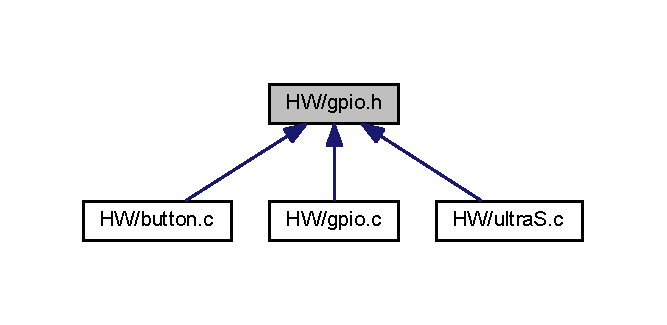
\includegraphics[width=320pt]{gpio_8h__dep__incl}
\end{center}
\end{figure}
\subsection*{Macros}
\begin{DoxyCompactItemize}
\item 
\#define \hyperlink{gpio_8h_ae952a5196156d96628c1e91f057fa182}{gpio\+\_\+get\+Pin\+Input}(port,  pin)~G\+P\+I\+O\+\_\+get\+Input\+Pin\+Value(port, pin)
\begin{DoxyCompactList}\small\item\em Sets local gpio to appropriate board function of similar name. \end{DoxyCompactList}\item 
\#define \hyperlink{gpio_8h_a335097c54e37a27dda7744bb26e9c003}{gpio\+\_\+set\+Pin\+High}(port,  pin)~G\+P\+I\+O\+\_\+set\+Output\+High\+On\+Pin(port, pin)
\begin{DoxyCompactList}\small\item\em Sets local gpio to appropriate board function of similar name. \end{DoxyCompactList}\item 
\#define \hyperlink{gpio_8h_a9ee956f33908b93898e82301b9a1b2c1}{gpio\+\_\+set\+Pin\+Low}(port,  pin)~G\+P\+I\+O\+\_\+set\+Output\+Low\+On\+Pin(port, pin)
\begin{DoxyCompactList}\small\item\em Sets local gpio to appropriate board function of similar name. \end{DoxyCompactList}\item 
\#define \hyperlink{gpio_8h_a41e2274d7895a0d405af1938c849dc76}{gpio\+\_\+get\+Interrupt}(port,  pin)~G\+P\+I\+O\+\_\+get\+Interrupt\+Status(port, pin)
\begin{DoxyCompactList}\small\item\em Sets local gpio to appropriate board function of similar name. \end{DoxyCompactList}\item 
\#define \hyperlink{gpio_8h_af6ca6ac27e29c175d0fc1f59e4478984}{gpio\+\_\+set\+Interrupt\+Edge}(port,  pin,  edge)~G\+P\+I\+O\+\_\+select\+Interrupt\+Edge(port, pin, edge)
\begin{DoxyCompactList}\small\item\em Sets local gpio to appropriate board function of similar name. \end{DoxyCompactList}\item 
\#define \hyperlink{gpio_8h_abbd3d2cc6720be19186b1262f2e4c11b}{gpio\+\_\+clear\+Interrupt}(port,  pin)~G\+P\+I\+O\+\_\+clear\+Interrupt(port, pin)
\begin{DoxyCompactList}\small\item\em Sets local gpio to appropriate board function of similar name. \end{DoxyCompactList}\item 
\hypertarget{gpio_8h_aa8c089270a0e14242fd3f9bc69c9e285}{}\label{gpio_8h_aa8c089270a0e14242fd3f9bc69c9e285} 
\#define {\bfseries gpio\+\_\+\+P\+O\+R\+T\+\_\+\+P1}~G\+P\+I\+O\+\_\+\+P\+O\+R\+T\+\_\+\+P1
\item 
\hypertarget{gpio_8h_abdd76f3472e61231f433bd4103bb77dc}{}\label{gpio_8h_abdd76f3472e61231f433bd4103bb77dc} 
\#define {\bfseries gpio\+\_\+\+P\+O\+R\+T\+\_\+\+P2}~G\+P\+I\+O\+\_\+\+P\+O\+R\+T\+\_\+\+P2
\item 
\hypertarget{gpio_8h_aa287ef5bb605aaadbf946c40ffd1dc20}{}\label{gpio_8h_aa287ef5bb605aaadbf946c40ffd1dc20} 
\#define {\bfseries gpio\+\_\+\+P\+O\+R\+T\+\_\+\+P3}~G\+P\+I\+O\+\_\+\+P\+O\+R\+T\+\_\+\+P3
\item 
\hypertarget{gpio_8h_a104a4bb6b885217c55d4bf8c6d906005}{}\label{gpio_8h_a104a4bb6b885217c55d4bf8c6d906005} 
\#define {\bfseries gpio\+\_\+\+P\+O\+R\+T\+\_\+\+P4}~G\+P\+I\+O\+\_\+\+P\+O\+R\+T\+\_\+\+P4
\item 
\hypertarget{gpio_8h_a5857a2e7155c08273a00be2833ebfb2e}{}\label{gpio_8h_a5857a2e7155c08273a00be2833ebfb2e} 
\#define {\bfseries gpio\+\_\+\+P\+O\+R\+T\+\_\+\+P5}~G\+P\+I\+O\+\_\+\+P\+O\+R\+T\+\_\+\+P5
\item 
\hypertarget{gpio_8h_af6194c3039fdaa1f64a9e7db82aa5ad0}{}\label{gpio_8h_af6194c3039fdaa1f64a9e7db82aa5ad0} 
\#define {\bfseries gpio\+\_\+\+P\+O\+R\+T\+\_\+\+P6}~G\+P\+I\+O\+\_\+\+P\+O\+R\+T\+\_\+\+P6
\item 
\hypertarget{gpio_8h_a80b8382f76a6ce2759ecd3bf9d0ae2d3}{}\label{gpio_8h_a80b8382f76a6ce2759ecd3bf9d0ae2d3} 
\#define {\bfseries gpio\+\_\+\+P\+O\+R\+T\+\_\+\+P7}~G\+P\+I\+O\+\_\+\+P\+O\+R\+T\+\_\+\+P7
\item 
\hypertarget{gpio_8h_a04e603ac15253a2360a421f3b715eae0}{}\label{gpio_8h_a04e603ac15253a2360a421f3b715eae0} 
\#define {\bfseries gpio\+\_\+\+P\+O\+R\+T\+\_\+\+P8}~G\+P\+I\+O\+\_\+\+P\+O\+R\+T\+\_\+\+P8
\item 
\hypertarget{gpio_8h_a4106da468a38592775a8da0722224e40}{}\label{gpio_8h_a4106da468a38592775a8da0722224e40} 
\#define {\bfseries gpio\+\_\+\+P\+O\+R\+T\+\_\+\+P9}~G\+P\+I\+O\+\_\+\+P\+O\+R\+T\+\_\+\+P9
\item 
\hypertarget{gpio_8h_ad108084ea90b5deee6cf1023c0fe3eca}{}\label{gpio_8h_ad108084ea90b5deee6cf1023c0fe3eca} 
\#define {\bfseries gpio\+\_\+\+P\+O\+R\+T\+\_\+\+P10}~G\+P\+I\+O\+\_\+\+P\+O\+R\+T\+\_\+\+P10
\item 
\hypertarget{gpio_8h_a2f224d1cede757dd4a14e198302f8d67}{}\label{gpio_8h_a2f224d1cede757dd4a14e198302f8d67} 
\#define {\bfseries gpio\+\_\+\+P\+O\+R\+T\+\_\+\+P11}~G\+P\+I\+O\+\_\+\+P\+O\+R\+T\+\_\+\+P11
\item 
\hypertarget{gpio_8h_ab19ce5c5b5fb6860653a6e484abdcc14}{}\label{gpio_8h_ab19ce5c5b5fb6860653a6e484abdcc14} 
\#define {\bfseries gpio\+\_\+\+P\+O\+R\+T\+\_\+\+PA}~G\+P\+I\+O\+\_\+\+P\+O\+R\+T\+\_\+\+PA
\item 
\hypertarget{gpio_8h_ab9c094b1a0b32ce9a4661bf71e899d21}{}\label{gpio_8h_ab9c094b1a0b32ce9a4661bf71e899d21} 
\#define {\bfseries gpio\+\_\+\+P\+O\+R\+T\+\_\+\+PB}~G\+P\+I\+O\+\_\+\+P\+O\+R\+T\+\_\+\+PB
\item 
\hypertarget{gpio_8h_a31f4a6fee2aceebe14fcad786503c602}{}\label{gpio_8h_a31f4a6fee2aceebe14fcad786503c602} 
\#define {\bfseries gpio\+\_\+\+P\+O\+R\+T\+\_\+\+PC}~G\+P\+I\+O\+\_\+\+P\+O\+R\+T\+\_\+\+PC
\item 
\hypertarget{gpio_8h_a8b5b061fd627ed97bd66ac531be2abe0}{}\label{gpio_8h_a8b5b061fd627ed97bd66ac531be2abe0} 
\#define {\bfseries gpio\+\_\+\+P\+O\+R\+T\+\_\+\+PD}~G\+P\+I\+O\+\_\+\+P\+O\+R\+T\+\_\+\+PD
\item 
\hypertarget{gpio_8h_a67de93aaa7415e0ba41bda4f18ba61cf}{}\label{gpio_8h_a67de93aaa7415e0ba41bda4f18ba61cf} 
\#define {\bfseries gpio\+\_\+\+P\+O\+R\+T\+\_\+\+PE}~G\+P\+I\+O\+\_\+\+P\+O\+R\+T\+\_\+\+PE
\item 
\hypertarget{gpio_8h_a10efac0d898bccea13b152e9437bdcd5}{}\label{gpio_8h_a10efac0d898bccea13b152e9437bdcd5} 
\#define {\bfseries gpio\+\_\+\+P\+O\+R\+T\+\_\+\+PF}~G\+P\+I\+O\+\_\+\+P\+O\+R\+T\+\_\+\+PF
\item 
\hypertarget{gpio_8h_a71e9c9ac19f339ac6c1ce4488c1f83a1}{}\label{gpio_8h_a71e9c9ac19f339ac6c1ce4488c1f83a1} 
\#define {\bfseries gpio\+\_\+\+P\+O\+R\+T\+\_\+\+PJ}~G\+P\+I\+O\+\_\+\+P\+O\+R\+T\+\_\+\+PJ
\item 
\hypertarget{gpio_8h_a6ec1ed72136cb5058b1de626efe37a47}{}\label{gpio_8h_a6ec1ed72136cb5058b1de626efe37a47} 
\#define {\bfseries gpio\+\_\+\+P\+I\+N0}~G\+P\+I\+O\+\_\+\+P\+I\+N0
\item 
\hypertarget{gpio_8h_ab184665f11481b88e18cbe14aa631ee6}{}\label{gpio_8h_ab184665f11481b88e18cbe14aa631ee6} 
\#define {\bfseries gpio\+\_\+\+P\+I\+N1}~G\+P\+I\+O\+\_\+\+P\+I\+N1
\item 
\hypertarget{gpio_8h_a2c978b7d3cbb9222dccccf7f0faa539b}{}\label{gpio_8h_a2c978b7d3cbb9222dccccf7f0faa539b} 
\#define {\bfseries gpio\+\_\+\+P\+I\+N2}~G\+P\+I\+O\+\_\+\+P\+I\+N2
\item 
\hypertarget{gpio_8h_a72de9e6a9f55b125f3cbf28509dafcda}{}\label{gpio_8h_a72de9e6a9f55b125f3cbf28509dafcda} 
\#define {\bfseries gpio\+\_\+\+P\+I\+N3}~G\+P\+I\+O\+\_\+\+P\+I\+N3
\item 
\hypertarget{gpio_8h_a13abe583db09fd3ff3e50c6d4bc082df}{}\label{gpio_8h_a13abe583db09fd3ff3e50c6d4bc082df} 
\#define {\bfseries gpio\+\_\+\+P\+I\+N4}~G\+P\+I\+O\+\_\+\+P\+I\+N4
\item 
\hypertarget{gpio_8h_a00634bcf1edad3fb36d9d324472dd036}{}\label{gpio_8h_a00634bcf1edad3fb36d9d324472dd036} 
\#define {\bfseries gpio\+\_\+\+P\+I\+N5}~G\+P\+I\+O\+\_\+\+P\+I\+N5
\item 
\hypertarget{gpio_8h_a2850b140b065688c701164dca4d47045}{}\label{gpio_8h_a2850b140b065688c701164dca4d47045} 
\#define {\bfseries gpio\+\_\+\+P\+I\+N6}~G\+P\+I\+O\+\_\+\+P\+I\+N6
\item 
\hypertarget{gpio_8h_afcd5b8d2806df23addb0d081e22b587b}{}\label{gpio_8h_afcd5b8d2806df23addb0d081e22b587b} 
\#define {\bfseries gpio\+\_\+\+P\+I\+N7}~G\+P\+I\+O\+\_\+\+P\+I\+N7
\item 
\hypertarget{gpio_8h_a19ceda01f87c5ef54995c1495e91658c}{}\label{gpio_8h_a19ceda01f87c5ef54995c1495e91658c} 
\#define {\bfseries gpio\+\_\+\+P\+I\+N8}~G\+P\+I\+O\+\_\+\+P\+I\+N8
\item 
\hypertarget{gpio_8h_a90fda6164dbaf326d580035b597a5605}{}\label{gpio_8h_a90fda6164dbaf326d580035b597a5605} 
\#define {\bfseries gpio\+\_\+\+P\+I\+N9}~G\+P\+I\+O\+\_\+\+P\+I\+N9
\item 
\hypertarget{gpio_8h_a73f1cdbadcb1f6244777664ab400b24a}{}\label{gpio_8h_a73f1cdbadcb1f6244777664ab400b24a} 
\#define {\bfseries gpio\+\_\+\+P\+I\+N10}~G\+P\+I\+O\+\_\+\+P\+I\+N10
\item 
\hypertarget{gpio_8h_a77d9a80d8441a86e29891174b6dfb5d0}{}\label{gpio_8h_a77d9a80d8441a86e29891174b6dfb5d0} 
\#define {\bfseries gpio\+\_\+\+P\+I\+N11}~G\+P\+I\+O\+\_\+\+P\+I\+N11
\item 
\hypertarget{gpio_8h_a4b841b746dc5aac58bd08a9a98c2a30f}{}\label{gpio_8h_a4b841b746dc5aac58bd08a9a98c2a30f} 
\#define {\bfseries gpio\+\_\+\+P\+I\+N12}~G\+P\+I\+O\+\_\+\+P\+I\+N12
\item 
\hypertarget{gpio_8h_aace8feb3a5c8a20f3899288af16b47fa}{}\label{gpio_8h_aace8feb3a5c8a20f3899288af16b47fa} 
\#define {\bfseries gpio\+\_\+\+P\+I\+N13}~G\+P\+I\+O\+\_\+\+P\+I\+N13
\item 
\hypertarget{gpio_8h_a5062ea4824b225524105f66d1db72339}{}\label{gpio_8h_a5062ea4824b225524105f66d1db72339} 
\#define {\bfseries gpio\+\_\+\+P\+I\+N14}~G\+P\+I\+O\+\_\+\+P\+I\+N14
\item 
\hypertarget{gpio_8h_aab23aa24a17d554f4144583ab0354307}{}\label{gpio_8h_aab23aa24a17d554f4144583ab0354307} 
\#define {\bfseries gpio\+\_\+\+P\+I\+N15}~G\+P\+I\+O\+\_\+\+P\+I\+N15
\item 
\hypertarget{gpio_8h_a8d5a842c6e4aecfb08640ba5e3114e33}{}\label{gpio_8h_a8d5a842c6e4aecfb08640ba5e3114e33} 
\#define {\bfseries gpio\+\_\+\+P\+I\+N\+\_\+\+A\+L\+L8}~G\+P\+I\+O\+\_\+\+P\+I\+N\+\_\+\+A\+L\+L8
\item 
\hypertarget{gpio_8h_a5ef018dcc1d7c801c30588680a1a70e1}{}\label{gpio_8h_a5ef018dcc1d7c801c30588680a1a70e1} 
\#define {\bfseries gpio\+\_\+\+P\+I\+N\+\_\+\+A\+L\+L16}~G\+P\+I\+O\+\_\+\+P\+I\+N\+\_\+\+A\+L\+L16
\item 
\hypertarget{gpio_8h_add4814d694da99da636f5c5360869f6b}{}\label{gpio_8h_add4814d694da99da636f5c5360869f6b} 
\#define {\bfseries gpio\+\_\+\+H\+I\+G\+H\+\_\+\+T\+O\+\_\+\+L\+O\+W\+\_\+\+T\+R\+A\+N\+S\+I\+T\+I\+ON}~G\+P\+I\+O\+\_\+\+H\+I\+G\+H\+\_\+\+T\+O\+\_\+\+L\+O\+W\+\_\+\+T\+R\+A\+N\+S\+I\+T\+I\+ON
\item 
\hypertarget{gpio_8h_ae94e2418b91bc671d102eda459367920}{}\label{gpio_8h_ae94e2418b91bc671d102eda459367920} 
\#define {\bfseries gpio\+\_\+\+L\+O\+W\+\_\+\+T\+O\+\_\+\+H\+I\+G\+H\+\_\+\+T\+R\+A\+N\+S\+I\+T\+I\+ON}~G\+P\+I\+O\+\_\+\+L\+O\+W\+\_\+\+T\+O\+\_\+\+H\+I\+G\+H\+\_\+\+T\+R\+A\+N\+S\+I\+T\+I\+ON
\end{DoxyCompactItemize}


\subsection{Macro Definition Documentation}
\hypertarget{gpio_8h_abbd3d2cc6720be19186b1262f2e4c11b}{}\label{gpio_8h_abbd3d2cc6720be19186b1262f2e4c11b} 
\index{gpio.\+h@{gpio.\+h}!gpio\+\_\+clear\+Interrupt@{gpio\+\_\+clear\+Interrupt}}
\index{gpio\+\_\+clear\+Interrupt@{gpio\+\_\+clear\+Interrupt}!gpio.\+h@{gpio.\+h}}
\subsubsection{\texorpdfstring{gpio\+\_\+clear\+Interrupt}{gpio\_clearInterrupt}}
{\footnotesize\ttfamily \#define gpio\+\_\+clear\+Interrupt(\begin{DoxyParamCaption}\item[{}]{port,  }\item[{}]{pin }\end{DoxyParamCaption})~G\+P\+I\+O\+\_\+clear\+Interrupt(port, pin)}



Sets local gpio to appropriate board function of similar name. 

Used to clear serviced interrupts on {\bfseries port\textquotesingle{}s} {\bfseries pin} \hypertarget{gpio_8h_a41e2274d7895a0d405af1938c849dc76}{}\label{gpio_8h_a41e2274d7895a0d405af1938c849dc76} 
\index{gpio.\+h@{gpio.\+h}!gpio\+\_\+get\+Interrupt@{gpio\+\_\+get\+Interrupt}}
\index{gpio\+\_\+get\+Interrupt@{gpio\+\_\+get\+Interrupt}!gpio.\+h@{gpio.\+h}}
\subsubsection{\texorpdfstring{gpio\+\_\+get\+Interrupt}{gpio\_getInterrupt}}
{\footnotesize\ttfamily \#define gpio\+\_\+get\+Interrupt(\begin{DoxyParamCaption}\item[{}]{port,  }\item[{}]{pin }\end{DoxyParamCaption})~G\+P\+I\+O\+\_\+get\+Interrupt\+Status(port, pin)}



Sets local gpio to appropriate board function of similar name. 

Gets {\bfseries port} {\bfseries pin\textquotesingle{}s} pending interrupt status.

Sets {\bfseries port\textquotesingle{}s} pin to a logical 1 \hypertarget{gpio_8h_ae952a5196156d96628c1e91f057fa182}{}\label{gpio_8h_ae952a5196156d96628c1e91f057fa182} 
\index{gpio.\+h@{gpio.\+h}!gpio\+\_\+get\+Pin\+Input@{gpio\+\_\+get\+Pin\+Input}}
\index{gpio\+\_\+get\+Pin\+Input@{gpio\+\_\+get\+Pin\+Input}!gpio.\+h@{gpio.\+h}}
\subsubsection{\texorpdfstring{gpio\+\_\+get\+Pin\+Input}{gpio\_getPinInput}}
{\footnotesize\ttfamily \#define gpio\+\_\+get\+Pin\+Input(\begin{DoxyParamCaption}\item[{}]{port,  }\item[{}]{pin }\end{DoxyParamCaption})~G\+P\+I\+O\+\_\+get\+Input\+Pin\+Value(port, pin)}



Sets local gpio to appropriate board function of similar name. 

Gets {\bfseries port} {\bfseries pin\textquotesingle{}s} logical value. \hypertarget{gpio_8h_af6ca6ac27e29c175d0fc1f59e4478984}{}\label{gpio_8h_af6ca6ac27e29c175d0fc1f59e4478984} 
\index{gpio.\+h@{gpio.\+h}!gpio\+\_\+set\+Interrupt\+Edge@{gpio\+\_\+set\+Interrupt\+Edge}}
\index{gpio\+\_\+set\+Interrupt\+Edge@{gpio\+\_\+set\+Interrupt\+Edge}!gpio.\+h@{gpio.\+h}}
\subsubsection{\texorpdfstring{gpio\+\_\+set\+Interrupt\+Edge}{gpio\_setInterruptEdge}}
{\footnotesize\ttfamily \#define gpio\+\_\+set\+Interrupt\+Edge(\begin{DoxyParamCaption}\item[{}]{port,  }\item[{}]{pin,  }\item[{}]{edge }\end{DoxyParamCaption})~G\+P\+I\+O\+\_\+select\+Interrupt\+Edge(port, pin, edge)}



Sets local gpio to appropriate board function of similar name. 

Sets {\bfseries port\textquotesingle{}s} {\bfseries pin} interrupt status to be set by either a falling or a rising edge. \hypertarget{gpio_8h_a335097c54e37a27dda7744bb26e9c003}{}\label{gpio_8h_a335097c54e37a27dda7744bb26e9c003} 
\index{gpio.\+h@{gpio.\+h}!gpio\+\_\+set\+Pin\+High@{gpio\+\_\+set\+Pin\+High}}
\index{gpio\+\_\+set\+Pin\+High@{gpio\+\_\+set\+Pin\+High}!gpio.\+h@{gpio.\+h}}
\subsubsection{\texorpdfstring{gpio\+\_\+set\+Pin\+High}{gpio\_setPinHigh}}
{\footnotesize\ttfamily \#define gpio\+\_\+set\+Pin\+High(\begin{DoxyParamCaption}\item[{}]{port,  }\item[{}]{pin }\end{DoxyParamCaption})~G\+P\+I\+O\+\_\+set\+Output\+High\+On\+Pin(port, pin)}



Sets local gpio to appropriate board function of similar name. 

Sets {\bfseries port\textquotesingle{}s} {\bfseries pin} to a logical 1 \hypertarget{gpio_8h_a9ee956f33908b93898e82301b9a1b2c1}{}\label{gpio_8h_a9ee956f33908b93898e82301b9a1b2c1} 
\index{gpio.\+h@{gpio.\+h}!gpio\+\_\+set\+Pin\+Low@{gpio\+\_\+set\+Pin\+Low}}
\index{gpio\+\_\+set\+Pin\+Low@{gpio\+\_\+set\+Pin\+Low}!gpio.\+h@{gpio.\+h}}
\subsubsection{\texorpdfstring{gpio\+\_\+set\+Pin\+Low}{gpio\_setPinLow}}
{\footnotesize\ttfamily \#define gpio\+\_\+set\+Pin\+Low(\begin{DoxyParamCaption}\item[{}]{port,  }\item[{}]{pin }\end{DoxyParamCaption})~G\+P\+I\+O\+\_\+set\+Output\+Low\+On\+Pin(port, pin)}



Sets local gpio to appropriate board function of similar name. 

Sets {\bfseries port\textquotesingle{}s} {\bfseries pin} to a logical 0 
\hypertarget{ultra_s_8c}{}\section{H\+W/ultraS.c File Reference}
\label{ultra_s_8c}\index{H\+W/ultra\+S.\+c@{H\+W/ultra\+S.\+c}}


\subsection{Detailed Description}
Documentation for the ultrasonic module. 

Describes the workings of the ultrasonic module.


\begin{DoxyImageNoCaption}
  \mbox{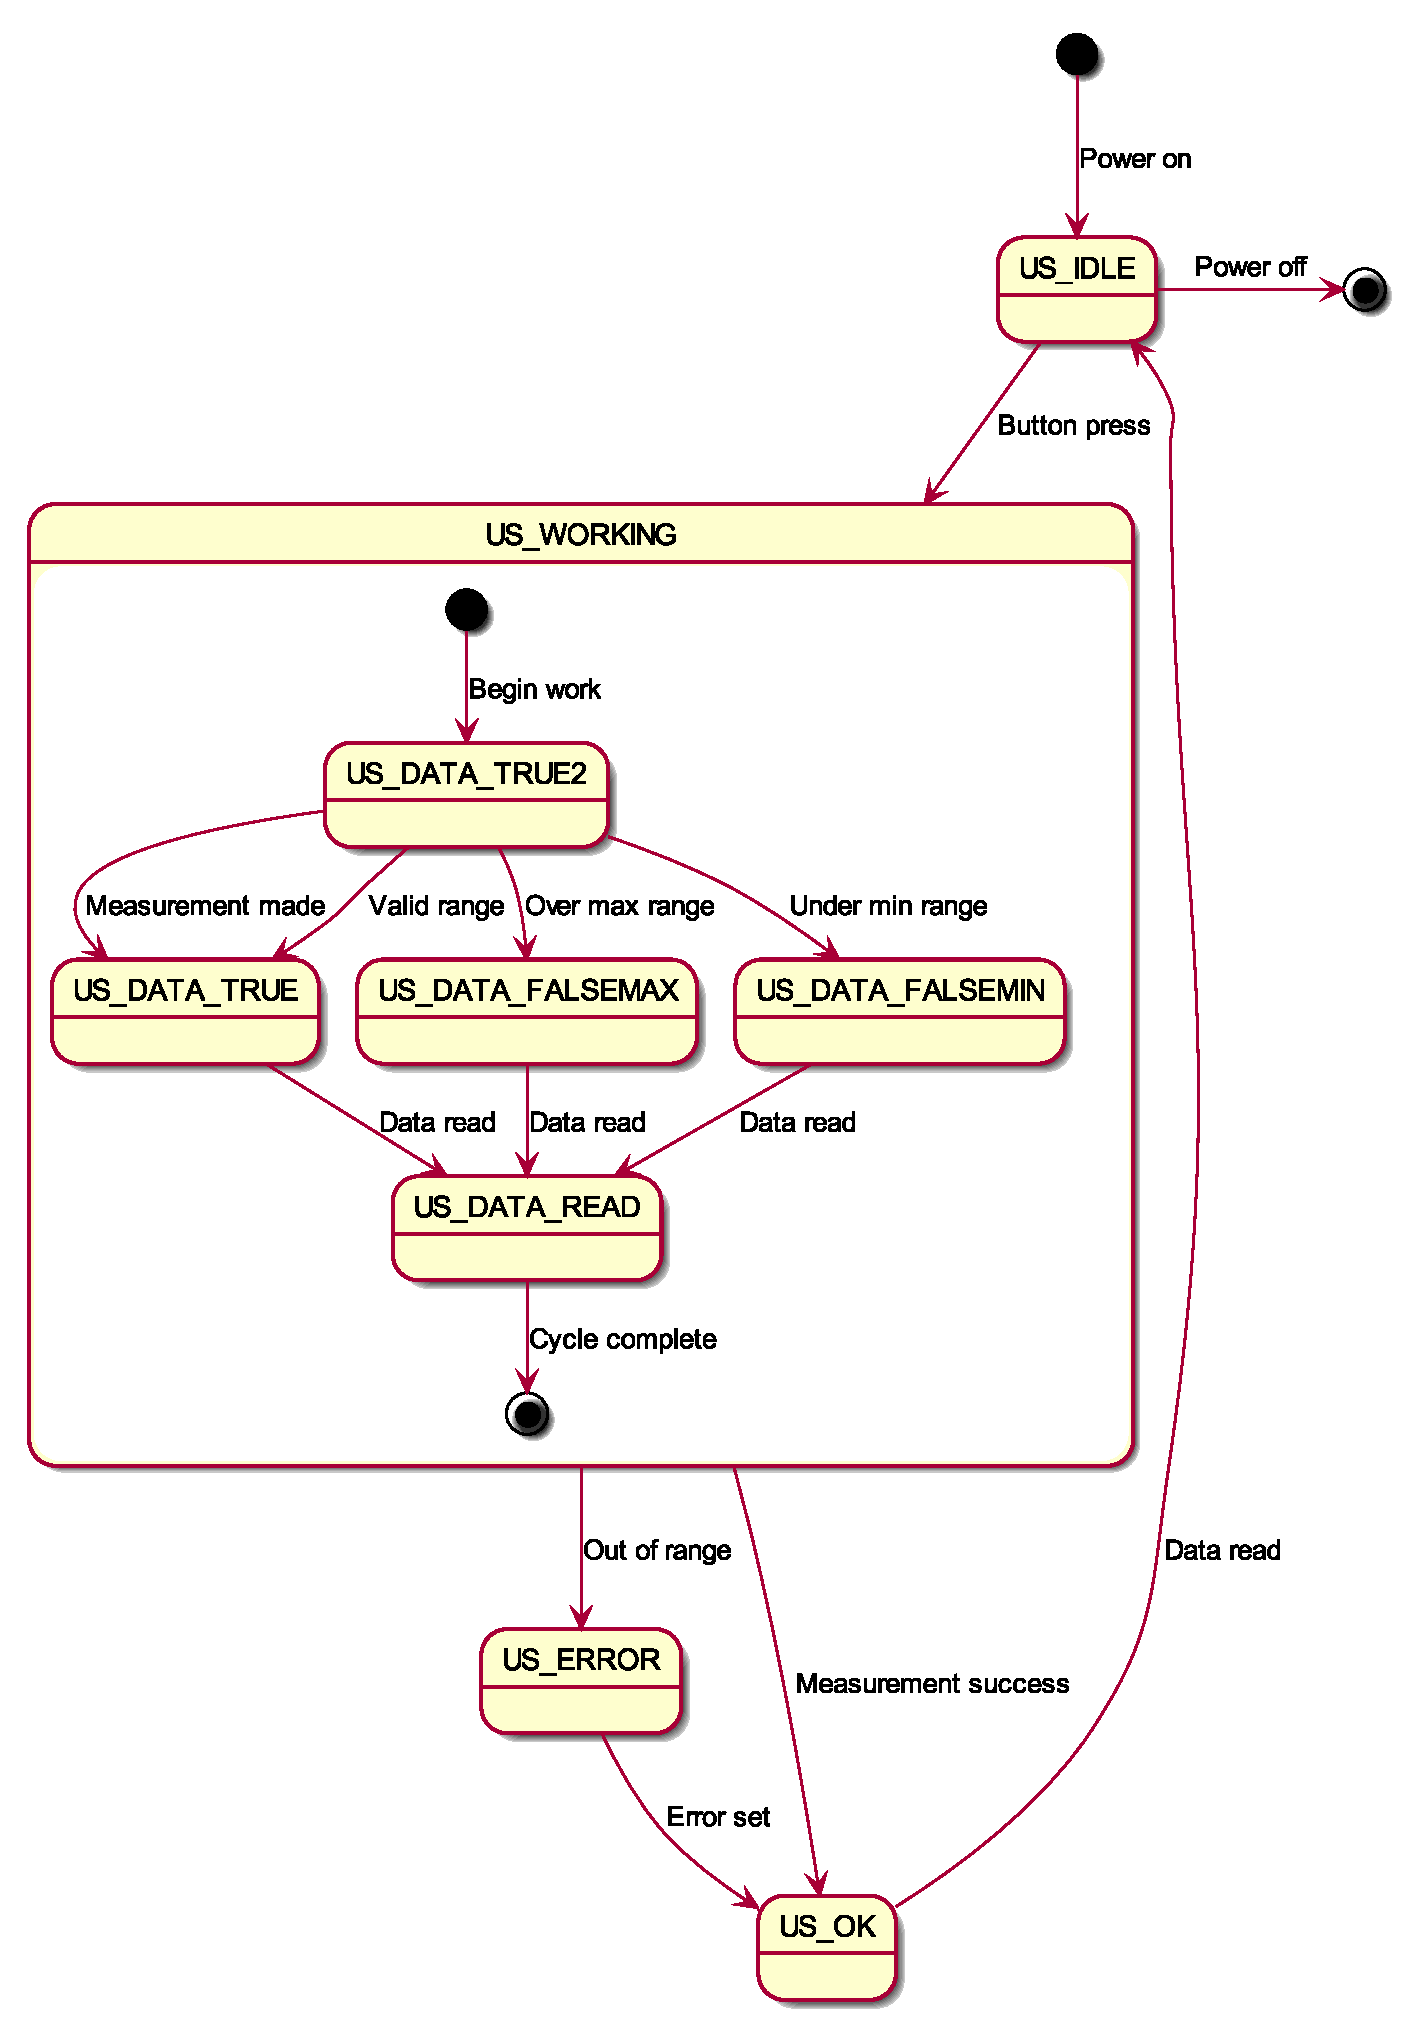
\includegraphics[width=\textwidth,height=\textheight/2,keepaspectratio=true]{umlFSM}}
\end{DoxyImageNoCaption}
 Include dependency graph for ultra\+S.\+c\+:\nopagebreak
\begin{figure}[H]
\begin{center}
\leavevmode
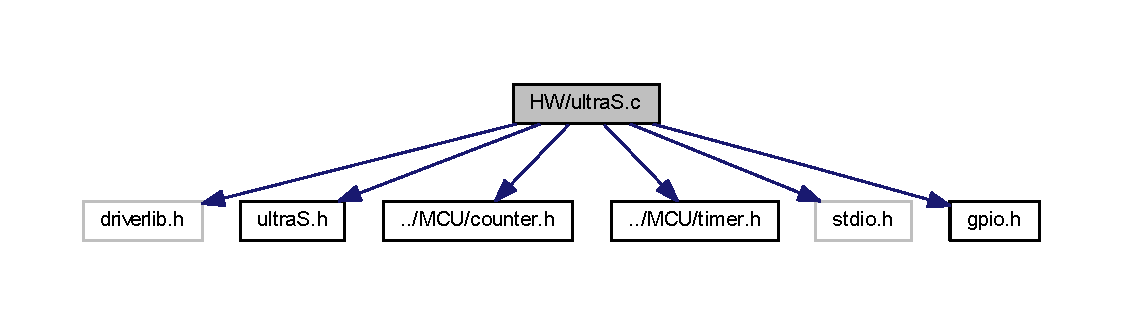
\includegraphics[width=350pt]{ultra_s_8c__incl}
\end{center}
\end{figure}
\subsection*{Macros}
\begin{DoxyCompactItemize}
\item 
\#define \hyperlink{ultra_s_8c_ad20257241c97c3e731b64608dcdc5096}{M\+A\+X\+D\+I\+ST}~23200
\item 
\#define \hyperlink{ultra_s_8c_abd40c30aeb838e9729fd6ebd4c4787d8}{M\+I\+N\+D\+I\+ST}~116
\item 
\#define \hyperlink{ultra_s_8c_a0212ca8fac649015507d58329b4e2cfc}{C\+M\+C\+O\+N\+ST}~58
\item 
\#define \hyperlink{ultra_s_8c_a78e81cc81d968960cf6089af8c033769}{C\+Y\+C\+LE}~0x\+F\+D\+E8
\end{DoxyCompactItemize}
\subsection*{Functions}
\begin{DoxyCompactItemize}
\item 
void \hyperlink{ultra_s_8c_afded4b6fd641aaf196a2bf062b82615d}{reset\+Times} ()
\item 
void \hyperlink{ultra_s_8c_a76007e39c7b3397710dee9bab7b5d9b5}{ultra\+S\+\_\+init} ()
\item 
void \hyperlink{ultra_s_8c_a2dc7671dcfab4e1cb316c3443f709a85}{ultra\+S\+\_\+send\+Signal} ()
\item 
void \hyperlink{ultra_s_8c_acdff37f2f4e581b47645303906a09417}{ultra\+S\+\_\+prep\+Info} ()
\item 
void \hyperlink{ultra_s_8c_a186e138633dbd47cca8dec6f41f86fb4}{ultra\+S\+\_\+cyclic} ()
\item 
unsigned int \hyperlink{ultra_s_8c_a85065971712e1812bab36f1366bc0416}{ultra\+S\+\_\+get\+Valid\+Status} ()
\item 
void \hyperlink{ultra_s_8c_a1030b82552b283571261c0977872f329}{ultra\+S\+\_\+set\+Valid\+Status} (\hyperlink{ultra_s_8h_a015eb90e0de9f16e87bd149d4b9ce959}{status} valid\+Status)
\item 
unsigned int \hyperlink{ultra_s_8c_ac80c09ba6b899105f44bdfe0be849296}{ultra\+S\+\_\+get\+Distance} ()
\item 
int \hyperlink{ultra_s_8c_ad5c0f2f041f3985396910a4b8c325b2a}{ultra\+S\+\_\+get\+Data\+Status} ()
\item 
void \hyperlink{ultra_s_8c_a905d422d987ede5de76032575870b0f9}{ultra\+S\+\_\+set\+Data\+Status} (\hyperlink{ultra_s_8h_a5af22166e4d97bfcc7589baec25bec7b}{data\+Status} valid\+Status)
\item 
\+\_\+\+\_\+interrupt void \hyperlink{ultra_s_8c_aa8c3f90478a445d776dff99fc0c98b57}{ultra\+S\+\_\+\+I\+SR} (void)
\end{DoxyCompactItemize}
\subsection*{Variables}
\begin{DoxyCompactItemize}
\item 
unsigned volatile long long int \hyperlink{ultra_s_8c_a844b54572135dff378b658bd65221263}{start\+Time}
\item 
unsigned volatile long long int \hyperlink{ultra_s_8c_a5abce346ccd3cad73218a5938c205e7d}{end\+Time}
\item 
unsigned volatile long long int \hyperlink{ultra_s_8c_a349cd5cafa77914b2cc6166055010c9b}{start\+Time\+Mult}
\item 
unsigned volatile long long int \hyperlink{ultra_s_8c_a6221a55ce2abd90d7398b6199cd179c4}{end\+Time\+Mult}
\item 
unsigned volatile long int \hyperlink{ultra_s_8c_a71ff771a4087c8674a0fa6720182d23f}{distance}
\item 
\hyperlink{ultra_s_8h_a015eb90e0de9f16e87bd149d4b9ce959}{status} \hyperlink{ultra_s_8c_a48b9dc63ee68bf7aee75f129d6631678}{us\+Status} = \hyperlink{ultra_s_8h_a015eb90e0de9f16e87bd149d4b9ce959a4444eecc516e45f891e67e9278efd311}{U\+S\+\_\+\+I\+D\+LE}
\item 
\hyperlink{ultra_s_8h_a5af22166e4d97bfcc7589baec25bec7b}{data\+Status} \hyperlink{ultra_s_8c_a211460b7d3250f3d56a6944d1f516858}{us\+Data\+Status} = \hyperlink{ultra_s_8h_a5af22166e4d97bfcc7589baec25bec7bae27f17d8a7ef52a5d6d5b8c4e562d453}{U\+S\+\_\+\+D\+A\+T\+A\+\_\+\+F\+A\+L\+SE}
\end{DoxyCompactItemize}


\subsection{Macro Definition Documentation}
\hypertarget{ultra_s_8c_a0212ca8fac649015507d58329b4e2cfc}{}\label{ultra_s_8c_a0212ca8fac649015507d58329b4e2cfc} 
\index{ultra\+S.\+c@{ultra\+S.\+c}!C\+M\+C\+O\+N\+ST@{C\+M\+C\+O\+N\+ST}}
\index{C\+M\+C\+O\+N\+ST@{C\+M\+C\+O\+N\+ST}!ultra\+S.\+c@{ultra\+S.\+c}}
\subsubsection{\texorpdfstring{C\+M\+C\+O\+N\+ST}{CMCONST}}
{\footnotesize\ttfamily \#define C\+M\+C\+O\+N\+ST~58}

Constant to divide time with to get distance in centimeters. \hypertarget{ultra_s_8c_a78e81cc81d968960cf6089af8c033769}{}\label{ultra_s_8c_a78e81cc81d968960cf6089af8c033769} 
\index{ultra\+S.\+c@{ultra\+S.\+c}!C\+Y\+C\+LE@{C\+Y\+C\+LE}}
\index{C\+Y\+C\+LE@{C\+Y\+C\+LE}!ultra\+S.\+c@{ultra\+S.\+c}}
\subsubsection{\texorpdfstring{C\+Y\+C\+LE}{CYCLE}}
{\footnotesize\ttfamily \#define C\+Y\+C\+LE~0x\+F\+D\+E8}

Timer size -\/ added to end\+Time when rollover happens. \hypertarget{ultra_s_8c_ad20257241c97c3e731b64608dcdc5096}{}\label{ultra_s_8c_ad20257241c97c3e731b64608dcdc5096} 
\index{ultra\+S.\+c@{ultra\+S.\+c}!M\+A\+X\+D\+I\+ST@{M\+A\+X\+D\+I\+ST}}
\index{M\+A\+X\+D\+I\+ST@{M\+A\+X\+D\+I\+ST}!ultra\+S.\+c@{ultra\+S.\+c}}
\subsubsection{\texorpdfstring{M\+A\+X\+D\+I\+ST}{MAXDIST}}
{\footnotesize\ttfamily \#define M\+A\+X\+D\+I\+ST~23200}

23200us is 4m. \hypertarget{ultra_s_8c_abd40c30aeb838e9729fd6ebd4c4787d8}{}\label{ultra_s_8c_abd40c30aeb838e9729fd6ebd4c4787d8} 
\index{ultra\+S.\+c@{ultra\+S.\+c}!M\+I\+N\+D\+I\+ST@{M\+I\+N\+D\+I\+ST}}
\index{M\+I\+N\+D\+I\+ST@{M\+I\+N\+D\+I\+ST}!ultra\+S.\+c@{ultra\+S.\+c}}
\subsubsection{\texorpdfstring{M\+I\+N\+D\+I\+ST}{MINDIST}}
{\footnotesize\ttfamily \#define M\+I\+N\+D\+I\+ST~116}

116us is 2cm. 

\subsection{Function Documentation}
\hypertarget{ultra_s_8c_afded4b6fd641aaf196a2bf062b82615d}{}\label{ultra_s_8c_afded4b6fd641aaf196a2bf062b82615d} 
\index{ultra\+S.\+c@{ultra\+S.\+c}!reset\+Times@{reset\+Times}}
\index{reset\+Times@{reset\+Times}!ultra\+S.\+c@{ultra\+S.\+c}}
\subsubsection{\texorpdfstring{reset\+Times()}{resetTimes()}}
{\footnotesize\ttfamily void reset\+Times (\begin{DoxyParamCaption}{ }\end{DoxyParamCaption})}

Reset start and end time to 0 to insure proper results. \begin{DoxyAttention}{Attention}
Private function. 
\end{DoxyAttention}
Here is the caller graph for this function\+:\nopagebreak
\begin{figure}[H]
\begin{center}
\leavevmode
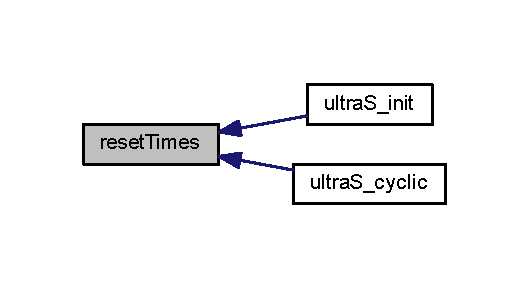
\includegraphics[width=254pt]{ultra_s_8c_afded4b6fd641aaf196a2bf062b82615d_icgraph}
\end{center}
\end{figure}
\hypertarget{ultra_s_8c_a186e138633dbd47cca8dec6f41f86fb4}{}\label{ultra_s_8c_a186e138633dbd47cca8dec6f41f86fb4} 
\index{ultra\+S.\+c@{ultra\+S.\+c}!ultra\+S\+\_\+cyclic@{ultra\+S\+\_\+cyclic}}
\index{ultra\+S\+\_\+cyclic@{ultra\+S\+\_\+cyclic}!ultra\+S.\+c@{ultra\+S.\+c}}
\subsubsection{\texorpdfstring{ultra\+S\+\_\+cyclic()}{ultraS\_cyclic()}}
{\footnotesize\ttfamily void ultra\+S\+\_\+cyclic (\begin{DoxyParamCaption}{ }\end{DoxyParamCaption})}

Ultrasonic modules main finite state machine.

Controls the work regarding the ultrasonic hardware. Finite state machine to decide state of system. \begin{DoxyAttention}{Attention}
U\+S\+\_\+\+W\+O\+R\+K\+I\+NG state is further controlled by another state machine. 
\end{DoxyAttention}
Here is the call graph for this function\+:\nopagebreak
\begin{figure}[H]
\begin{center}
\leavevmode
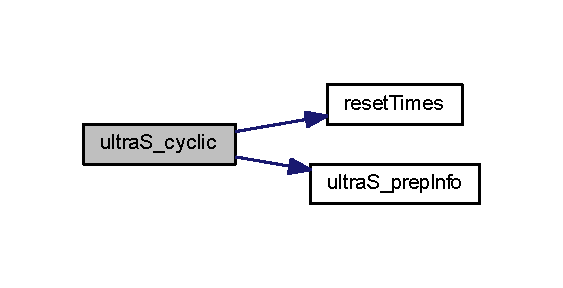
\includegraphics[width=270pt]{ultra_s_8c_a186e138633dbd47cca8dec6f41f86fb4_cgraph}
\end{center}
\end{figure}
\hypertarget{ultra_s_8c_ad5c0f2f041f3985396910a4b8c325b2a}{}\label{ultra_s_8c_ad5c0f2f041f3985396910a4b8c325b2a} 
\index{ultra\+S.\+c@{ultra\+S.\+c}!ultra\+S\+\_\+get\+Data\+Status@{ultra\+S\+\_\+get\+Data\+Status}}
\index{ultra\+S\+\_\+get\+Data\+Status@{ultra\+S\+\_\+get\+Data\+Status}!ultra\+S.\+c@{ultra\+S.\+c}}
\subsubsection{\texorpdfstring{ultra\+S\+\_\+get\+Data\+Status()}{ultraS\_getDataStatus()}}
{\footnotesize\ttfamily int ultra\+S\+\_\+get\+Data\+Status (\begin{DoxyParamCaption}{ }\end{DoxyParamCaption})}

Get ultrasonic modules workings state.

Get the inner F\+SM\textquotesingle{}s state. \begin{DoxyReturn}{Returns}
us\+Data\+Status
\end{DoxyReturn}
Here is the caller graph for this function\+:\nopagebreak
\begin{figure}[H]
\begin{center}
\leavevmode
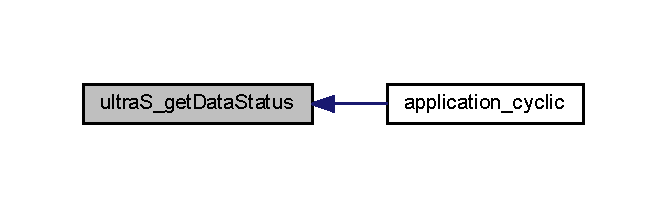
\includegraphics[width=320pt]{ultra_s_8c_ad5c0f2f041f3985396910a4b8c325b2a_icgraph}
\end{center}
\end{figure}
\hypertarget{ultra_s_8c_ac80c09ba6b899105f44bdfe0be849296}{}\label{ultra_s_8c_ac80c09ba6b899105f44bdfe0be849296} 
\index{ultra\+S.\+c@{ultra\+S.\+c}!ultra\+S\+\_\+get\+Distance@{ultra\+S\+\_\+get\+Distance}}
\index{ultra\+S\+\_\+get\+Distance@{ultra\+S\+\_\+get\+Distance}!ultra\+S.\+c@{ultra\+S.\+c}}
\subsubsection{\texorpdfstring{ultra\+S\+\_\+get\+Distance()}{ultraS\_getDistance()}}
{\footnotesize\ttfamily unsigned int ultra\+S\+\_\+get\+Distance (\begin{DoxyParamCaption}{ }\end{DoxyParamCaption})}

Get measured distance.

\begin{DoxyReturn}{Returns}
Distance 
\end{DoxyReturn}
Here is the caller graph for this function\+:\nopagebreak
\begin{figure}[H]
\begin{center}
\leavevmode
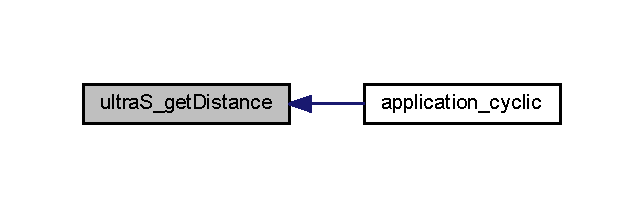
\includegraphics[width=309pt]{ultra_s_8c_ac80c09ba6b899105f44bdfe0be849296_icgraph}
\end{center}
\end{figure}
\hypertarget{ultra_s_8c_a85065971712e1812bab36f1366bc0416}{}\label{ultra_s_8c_a85065971712e1812bab36f1366bc0416} 
\index{ultra\+S.\+c@{ultra\+S.\+c}!ultra\+S\+\_\+get\+Valid\+Status@{ultra\+S\+\_\+get\+Valid\+Status}}
\index{ultra\+S\+\_\+get\+Valid\+Status@{ultra\+S\+\_\+get\+Valid\+Status}!ultra\+S.\+c@{ultra\+S.\+c}}
\subsubsection{\texorpdfstring{ultra\+S\+\_\+get\+Valid\+Status()}{ultraS\_getValidStatus()}}
{\footnotesize\ttfamily unsigned int ultra\+S\+\_\+get\+Valid\+Status (\begin{DoxyParamCaption}{ }\end{DoxyParamCaption})}

Get ultrasonic modules state.

\begin{DoxyReturn}{Returns}
us\+Status 
\end{DoxyReturn}
Here is the caller graph for this function\+:\nopagebreak
\begin{figure}[H]
\begin{center}
\leavevmode
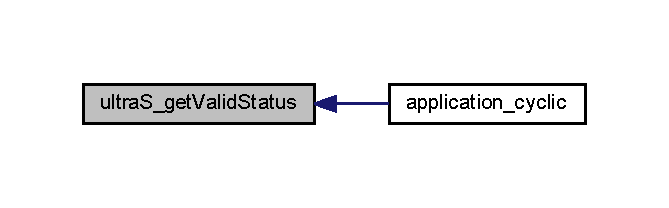
\includegraphics[width=321pt]{ultra_s_8c_a85065971712e1812bab36f1366bc0416_icgraph}
\end{center}
\end{figure}
\hypertarget{ultra_s_8c_a76007e39c7b3397710dee9bab7b5d9b5}{}\label{ultra_s_8c_a76007e39c7b3397710dee9bab7b5d9b5} 
\index{ultra\+S.\+c@{ultra\+S.\+c}!ultra\+S\+\_\+init@{ultra\+S\+\_\+init}}
\index{ultra\+S\+\_\+init@{ultra\+S\+\_\+init}!ultra\+S.\+c@{ultra\+S.\+c}}
\subsubsection{\texorpdfstring{ultra\+S\+\_\+init()}{ultraS\_init()}}
{\footnotesize\ttfamily void ultra\+S\+\_\+init (\begin{DoxyParamCaption}{ }\end{DoxyParamCaption})}

Set ultrasonic module to be ready for work.

Set\textquotesingle{}s appropriate F\+SM states and resets start and end times to 0. Here is the call graph for this function\+:\nopagebreak
\begin{figure}[H]
\begin{center}
\leavevmode
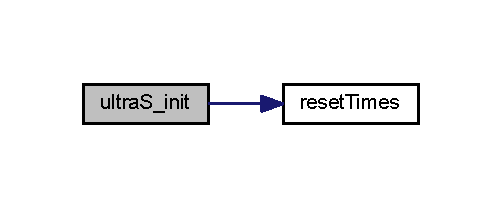
\includegraphics[width=241pt]{ultra_s_8c_a76007e39c7b3397710dee9bab7b5d9b5_cgraph}
\end{center}
\end{figure}
\hypertarget{ultra_s_8c_aa8c3f90478a445d776dff99fc0c98b57}{}\label{ultra_s_8c_aa8c3f90478a445d776dff99fc0c98b57} 
\index{ultra\+S.\+c@{ultra\+S.\+c}!ultra\+S\+\_\+\+I\+SR@{ultra\+S\+\_\+\+I\+SR}}
\index{ultra\+S\+\_\+\+I\+SR@{ultra\+S\+\_\+\+I\+SR}!ultra\+S.\+c@{ultra\+S.\+c}}
\subsubsection{\texorpdfstring{ultra\+S\+\_\+\+I\+S\+R()}{ultraS\_ISR()}}
{\footnotesize\ttfamily \+\_\+\+\_\+interrupt void ultra\+S\+\_\+\+I\+SR (\begin{DoxyParamCaption}\item[{void}]{ }\end{DoxyParamCaption})}

Interrupt vector for Port 1.

Is triggered when the hardware ultrasonic module sends back an echo signal. ~\newline
 The rising edge of the echo signal is saved as the starting time and the falling edge as the ending time. \hypertarget{ultra_s_8c_acdff37f2f4e581b47645303906a09417}{}\label{ultra_s_8c_acdff37f2f4e581b47645303906a09417} 
\index{ultra\+S.\+c@{ultra\+S.\+c}!ultra\+S\+\_\+prep\+Info@{ultra\+S\+\_\+prep\+Info}}
\index{ultra\+S\+\_\+prep\+Info@{ultra\+S\+\_\+prep\+Info}!ultra\+S.\+c@{ultra\+S.\+c}}
\subsubsection{\texorpdfstring{ultra\+S\+\_\+prep\+Info()}{ultraS\_prepInfo()}}
{\footnotesize\ttfamily void ultra\+S\+\_\+prep\+Info (\begin{DoxyParamCaption}{ }\end{DoxyParamCaption})}

Calculates measured distance.

Measured distance is calculated as\+: end time -\/ start time, which is then divided by 58 -\/ constant to get the distance in centimeters. ~\newline
 End time is the difference of the end and start time multiplier times the counter size added to the measured end time. Start time is just the measured start time. \begin{DoxyAttention}{Attention}
Only when rollover happens! 

Adds the entire counter size to end\+Time to compensate for potential rollover. 
\end{DoxyAttention}
Here is the caller graph for this function\+:\nopagebreak
\begin{figure}[H]
\begin{center}
\leavevmode
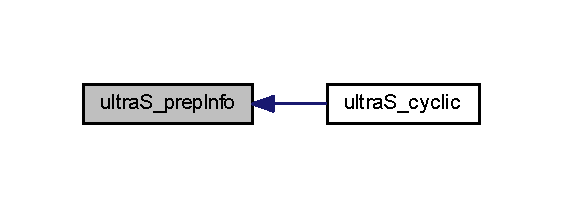
\includegraphics[width=270pt]{ultra_s_8c_acdff37f2f4e581b47645303906a09417_icgraph}
\end{center}
\end{figure}
\hypertarget{ultra_s_8c_a2dc7671dcfab4e1cb316c3443f709a85}{}\label{ultra_s_8c_a2dc7671dcfab4e1cb316c3443f709a85} 
\index{ultra\+S.\+c@{ultra\+S.\+c}!ultra\+S\+\_\+send\+Signal@{ultra\+S\+\_\+send\+Signal}}
\index{ultra\+S\+\_\+send\+Signal@{ultra\+S\+\_\+send\+Signal}!ultra\+S.\+c@{ultra\+S.\+c}}
\subsubsection{\texorpdfstring{ultra\+S\+\_\+send\+Signal()}{ultraS\_sendSignal()}}
{\footnotesize\ttfamily void ultra\+S\+\_\+send\+Signal (\begin{DoxyParamCaption}{ }\end{DoxyParamCaption})}

Send signal to the physical ultrasonic module.

Set\textquotesingle{}s appropriate F\+SM state. Send\textquotesingle{}s a high signal for required time -\/ 10uS. ~\newline
 Delays system to not send multiple signals at the same time. Here is the caller graph for this function\+:\nopagebreak
\begin{figure}[H]
\begin{center}
\leavevmode
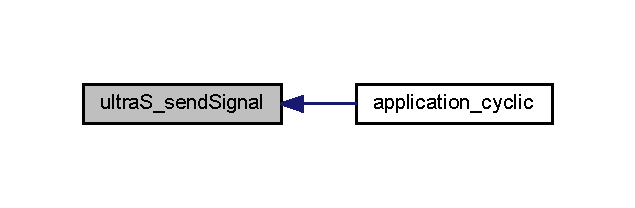
\includegraphics[width=305pt]{ultra_s_8c_a2dc7671dcfab4e1cb316c3443f709a85_icgraph}
\end{center}
\end{figure}
\hypertarget{ultra_s_8c_a905d422d987ede5de76032575870b0f9}{}\label{ultra_s_8c_a905d422d987ede5de76032575870b0f9} 
\index{ultra\+S.\+c@{ultra\+S.\+c}!ultra\+S\+\_\+set\+Data\+Status@{ultra\+S\+\_\+set\+Data\+Status}}
\index{ultra\+S\+\_\+set\+Data\+Status@{ultra\+S\+\_\+set\+Data\+Status}!ultra\+S.\+c@{ultra\+S.\+c}}
\subsubsection{\texorpdfstring{ultra\+S\+\_\+set\+Data\+Status()}{ultraS\_setDataStatus()}}
{\footnotesize\ttfamily void ultra\+S\+\_\+set\+Data\+Status (\begin{DoxyParamCaption}\item[{\hyperlink{ultra_s_8h_a5af22166e4d97bfcc7589baec25bec7b}{data\+Status}}]{valid\+Status }\end{DoxyParamCaption})}

Set ultrasonic modules workings state.

Set the inner F\+SM\textquotesingle{}s state. 
\begin{DoxyParams}{Parameters}
{\em valid\+Status} & Status to set \\
\hline
\end{DoxyParams}
Here is the caller graph for this function\+:\nopagebreak
\begin{figure}[H]
\begin{center}
\leavevmode
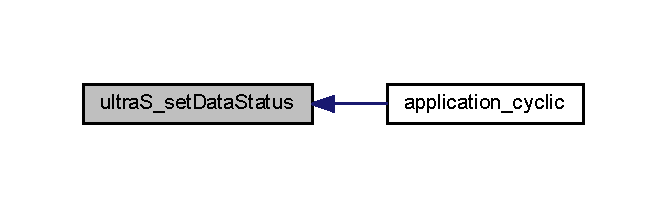
\includegraphics[width=320pt]{ultra_s_8c_a905d422d987ede5de76032575870b0f9_icgraph}
\end{center}
\end{figure}
\hypertarget{ultra_s_8c_a1030b82552b283571261c0977872f329}{}\label{ultra_s_8c_a1030b82552b283571261c0977872f329} 
\index{ultra\+S.\+c@{ultra\+S.\+c}!ultra\+S\+\_\+set\+Valid\+Status@{ultra\+S\+\_\+set\+Valid\+Status}}
\index{ultra\+S\+\_\+set\+Valid\+Status@{ultra\+S\+\_\+set\+Valid\+Status}!ultra\+S.\+c@{ultra\+S.\+c}}
\subsubsection{\texorpdfstring{ultra\+S\+\_\+set\+Valid\+Status()}{ultraS\_setValidStatus()}}
{\footnotesize\ttfamily void ultra\+S\+\_\+set\+Valid\+Status (\begin{DoxyParamCaption}\item[{\hyperlink{ultra_s_8h_a015eb90e0de9f16e87bd149d4b9ce959}{status}}]{valid\+Status }\end{DoxyParamCaption})}

Set ultrasonic modules state. 
\begin{DoxyParams}{Parameters}
{\em valid\+Status} & Status to set \\
\hline
\end{DoxyParams}


\subsection{Variable Documentation}
\hypertarget{ultra_s_8c_a71ff771a4087c8674a0fa6720182d23f}{}\label{ultra_s_8c_a71ff771a4087c8674a0fa6720182d23f} 
\index{ultra\+S.\+c@{ultra\+S.\+c}!distance@{distance}}
\index{distance@{distance}!ultra\+S.\+c@{ultra\+S.\+c}}
\subsubsection{\texorpdfstring{distance}{distance}}
{\footnotesize\ttfamily unsigned volatile long int distance}

Distance calculated based on start and end time and it\textquotesingle{}s multipliers \hypertarget{ultra_s_8c_a5abce346ccd3cad73218a5938c205e7d}{}\label{ultra_s_8c_a5abce346ccd3cad73218a5938c205e7d} 
\index{ultra\+S.\+c@{ultra\+S.\+c}!end\+Time@{end\+Time}}
\index{end\+Time@{end\+Time}!ultra\+S.\+c@{ultra\+S.\+c}}
\subsubsection{\texorpdfstring{end\+Time}{endTime}}
{\footnotesize\ttfamily unsigned volatile long long int end\+Time}

Time captured on usmodule\textquotesingle{}s falling edge echo signal. \hypertarget{ultra_s_8c_a6221a55ce2abd90d7398b6199cd179c4}{}\label{ultra_s_8c_a6221a55ce2abd90d7398b6199cd179c4} 
\index{ultra\+S.\+c@{ultra\+S.\+c}!end\+Time\+Mult@{end\+Time\+Mult}}
\index{end\+Time\+Mult@{end\+Time\+Mult}!ultra\+S.\+c@{ultra\+S.\+c}}
\subsubsection{\texorpdfstring{end\+Time\+Mult}{endTimeMult}}
{\footnotesize\ttfamily unsigned volatile long long int end\+Time\+Mult}

Insurance variable to insure that start\+Time and end\+Time are correct. \hypertarget{ultra_s_8c_a844b54572135dff378b658bd65221263}{}\label{ultra_s_8c_a844b54572135dff378b658bd65221263} 
\index{ultra\+S.\+c@{ultra\+S.\+c}!start\+Time@{start\+Time}}
\index{start\+Time@{start\+Time}!ultra\+S.\+c@{ultra\+S.\+c}}
\subsubsection{\texorpdfstring{start\+Time}{startTime}}
{\footnotesize\ttfamily unsigned volatile long long int start\+Time}

Time captured on usmodule\textquotesingle{}s rising edge echo signal. \hypertarget{ultra_s_8c_a349cd5cafa77914b2cc6166055010c9b}{}\label{ultra_s_8c_a349cd5cafa77914b2cc6166055010c9b} 
\index{ultra\+S.\+c@{ultra\+S.\+c}!start\+Time\+Mult@{start\+Time\+Mult}}
\index{start\+Time\+Mult@{start\+Time\+Mult}!ultra\+S.\+c@{ultra\+S.\+c}}
\subsubsection{\texorpdfstring{start\+Time\+Mult}{startTimeMult}}
{\footnotesize\ttfamily unsigned volatile long long int start\+Time\+Mult}

Insurance variable to insure that start\+Time and end\+Time are correct. \hypertarget{ultra_s_8c_a211460b7d3250f3d56a6944d1f516858}{}\label{ultra_s_8c_a211460b7d3250f3d56a6944d1f516858} 
\index{ultra\+S.\+c@{ultra\+S.\+c}!us\+Data\+Status@{us\+Data\+Status}}
\index{us\+Data\+Status@{us\+Data\+Status}!ultra\+S.\+c@{ultra\+S.\+c}}
\subsubsection{\texorpdfstring{us\+Data\+Status}{usDataStatus}}
{\footnotesize\ttfamily \hyperlink{ultra_s_8h_a5af22166e4d97bfcc7589baec25bec7b}{data\+Status} us\+Data\+Status = \hyperlink{ultra_s_8h_a5af22166e4d97bfcc7589baec25bec7bae27f17d8a7ef52a5d6d5b8c4e562d453}{U\+S\+\_\+\+D\+A\+T\+A\+\_\+\+F\+A\+L\+SE}}

Set finite state machine to start in false state to insure no false information. \hypertarget{ultra_s_8c_a48b9dc63ee68bf7aee75f129d6631678}{}\label{ultra_s_8c_a48b9dc63ee68bf7aee75f129d6631678} 
\index{ultra\+S.\+c@{ultra\+S.\+c}!us\+Status@{us\+Status}}
\index{us\+Status@{us\+Status}!ultra\+S.\+c@{ultra\+S.\+c}}
\subsubsection{\texorpdfstring{us\+Status}{usStatus}}
{\footnotesize\ttfamily \hyperlink{ultra_s_8h_a015eb90e0de9f16e87bd149d4b9ce959}{status} us\+Status = \hyperlink{ultra_s_8h_a015eb90e0de9f16e87bd149d4b9ce959a4444eecc516e45f891e67e9278efd311}{U\+S\+\_\+\+I\+D\+LE}}

Set finite state machine to idle/waiting state. 
\hypertarget{ultra_s_8h}{}\section{S\+R\+C/\+H\+W/ultraS.h File Reference}
\label{ultra_s_8h}\index{S\+R\+C/\+H\+W/ultra\+S.\+h@{S\+R\+C/\+H\+W/ultra\+S.\+h}}


Header file for the ultrasonic module.  


\subsection*{Enumerations}
\begin{DoxyCompactItemize}
\item 
enum \hyperlink{ultra_s_8h_a015eb90e0de9f16e87bd149d4b9ce959}{status} \{ \newline
\hyperlink{ultra_s_8h_a015eb90e0de9f16e87bd149d4b9ce959a688bb2aea3f560be00db855a2807e6fa}{U\+S\+\_\+\+OK}, 
\hyperlink{ultra_s_8h_a015eb90e0de9f16e87bd149d4b9ce959a8b86e148c08da560ab163c02be34254c}{U\+S\+\_\+\+W\+O\+R\+K\+I\+NG}, 
\hyperlink{ultra_s_8h_a015eb90e0de9f16e87bd149d4b9ce959a2fd3a96bffe618698f94b9308c9b4f51}{U\+S\+\_\+\+E\+R\+R\+OR}, 
\hyperlink{ultra_s_8h_a015eb90e0de9f16e87bd149d4b9ce959a4444eecc516e45f891e67e9278efd311}{U\+S\+\_\+\+I\+D\+LE}, 
\newline
{\bfseries U\+S\+\_\+\+N\+U\+M\+B\+E\+R\+\_\+\+O\+F\+\_\+\+T\+Y\+P\+ES}
 \}
\item 
enum \hyperlink{ultra_s_8h_a5af22166e4d97bfcc7589baec25bec7b}{data\+Status} \{ \newline
\hyperlink{ultra_s_8h_a5af22166e4d97bfcc7589baec25bec7ba2b0d9c232a242f02d30e512b8908b35a}{U\+S\+\_\+\+D\+A\+T\+A\+\_\+\+F\+A\+L\+S\+E\+M\+IN}, 
\hyperlink{ultra_s_8h_a5af22166e4d97bfcc7589baec25bec7bacc98738e6892bda59facfa3ad35aac69}{U\+S\+\_\+\+D\+A\+T\+A\+\_\+\+F\+A\+L\+S\+E\+M\+AX}, 
\hyperlink{ultra_s_8h_a5af22166e4d97bfcc7589baec25bec7bab4e04d20d63c362b5bba9b6125d34eee}{U\+S\+\_\+\+D\+A\+T\+A\+\_\+\+T\+R\+UE}, 
\hyperlink{ultra_s_8h_a5af22166e4d97bfcc7589baec25bec7ba2139ffa97370f4cb86ee95404d78ef7b}{U\+S\+\_\+\+D\+A\+T\+A\+\_\+\+T\+R\+U\+E2}, 
\newline
\hyperlink{ultra_s_8h_a5af22166e4d97bfcc7589baec25bec7bae27f17d8a7ef52a5d6d5b8c4e562d453}{U\+S\+\_\+\+D\+A\+T\+A\+\_\+\+F\+A\+L\+SE}, 
\hyperlink{ultra_s_8h_a5af22166e4d97bfcc7589baec25bec7ba50827340ffe4c961347eb0c3e601f3c4}{U\+S\+\_\+\+D\+A\+T\+A\+\_\+\+R\+E\+AD}, 
{\bfseries U\+S\+\_\+\+D\+A\+T\+A\+\_\+\+N\+U\+M\+B\+E\+R\+\_\+\+O\+F\+\_\+\+T\+Y\+P\+ES}
 \}
\end{DoxyCompactItemize}
\subsection*{Functions}
\begin{DoxyCompactItemize}
\item 
void \hyperlink{ultra_s_8h_a76007e39c7b3397710dee9bab7b5d9b5}{ultra\+S\+\_\+init} ()
\item 
void \hyperlink{ultra_s_8h_a2dc7671dcfab4e1cb316c3443f709a85}{ultra\+S\+\_\+send\+Signal} ()
\item 
void \hyperlink{ultra_s_8h_acdff37f2f4e581b47645303906a09417}{ultra\+S\+\_\+prep\+Info} ()
\item 
void \hyperlink{ultra_s_8h_a186e138633dbd47cca8dec6f41f86fb4}{ultra\+S\+\_\+cyclic} ()
\item 
unsigned int \hyperlink{ultra_s_8h_a85065971712e1812bab36f1366bc0416}{ultra\+S\+\_\+get\+Valid\+Status} ()
\item 
void \hyperlink{ultra_s_8h_a3aa336805b30c760503c3a2c9792d1b0}{ultra\+S\+\_\+set\+Valid\+Status} (enum \hyperlink{ultra_s_8h_a015eb90e0de9f16e87bd149d4b9ce959}{status} valid\+Status)
\item 
unsigned int \hyperlink{ultra_s_8h_ac80c09ba6b899105f44bdfe0be849296}{ultra\+S\+\_\+get\+Distance} ()
\item 
int \hyperlink{ultra_s_8h_ad5c0f2f041f3985396910a4b8c325b2a}{ultra\+S\+\_\+get\+Data\+Status} ()
\item 
void \hyperlink{ultra_s_8h_a8a5d4bdd11c244c8b0341256f5998d13}{ultra\+S\+\_\+set\+Data\+Status} (enum \hyperlink{ultra_s_8h_a5af22166e4d97bfcc7589baec25bec7b}{data\+Status} valid\+Status)
\end{DoxyCompactItemize}


\subsection{Detailed Description}
Header file for the ultrasonic module. 



\subsection{Enumeration Type Documentation}
\hypertarget{ultra_s_8h_a5af22166e4d97bfcc7589baec25bec7b}{}\label{ultra_s_8h_a5af22166e4d97bfcc7589baec25bec7b} 
\index{ultra\+S.\+h@{ultra\+S.\+h}!data\+Status@{data\+Status}}
\index{data\+Status@{data\+Status}!ultra\+S.\+h@{ultra\+S.\+h}}
\subsubsection{\texorpdfstring{data\+Status}{dataStatus}}
{\footnotesize\ttfamily enum \hyperlink{ultra_s_8h_a5af22166e4d97bfcc7589baec25bec7b}{data\+Status}}

\begin{DoxyEnumFields}{Enumerator}
\raisebox{\heightof{T}}[0pt][0pt]{\index{U\+S\+\_\+\+D\+A\+T\+A\+\_\+\+F\+A\+L\+S\+E\+M\+IN@{U\+S\+\_\+\+D\+A\+T\+A\+\_\+\+F\+A\+L\+S\+E\+M\+IN}!ultra\+S.\+h@{ultra\+S.\+h}}\index{ultra\+S.\+h@{ultra\+S.\+h}!U\+S\+\_\+\+D\+A\+T\+A\+\_\+\+F\+A\+L\+S\+E\+M\+IN@{U\+S\+\_\+\+D\+A\+T\+A\+\_\+\+F\+A\+L\+S\+E\+M\+IN}}}\hypertarget{ultra_s_8h_a5af22166e4d97bfcc7589baec25bec7ba2b0d9c232a242f02d30e512b8908b35a}{}\label{ultra_s_8h_a5af22166e4d97bfcc7589baec25bec7ba2b0d9c232a242f02d30e512b8908b35a} 
U\+S\+\_\+\+D\+A\+T\+A\+\_\+\+F\+A\+L\+S\+E\+M\+IN&Under the minimum 2cm distance. \\
\hline

\raisebox{\heightof{T}}[0pt][0pt]{\index{U\+S\+\_\+\+D\+A\+T\+A\+\_\+\+F\+A\+L\+S\+E\+M\+AX@{U\+S\+\_\+\+D\+A\+T\+A\+\_\+\+F\+A\+L\+S\+E\+M\+AX}!ultra\+S.\+h@{ultra\+S.\+h}}\index{ultra\+S.\+h@{ultra\+S.\+h}!U\+S\+\_\+\+D\+A\+T\+A\+\_\+\+F\+A\+L\+S\+E\+M\+AX@{U\+S\+\_\+\+D\+A\+T\+A\+\_\+\+F\+A\+L\+S\+E\+M\+AX}}}\hypertarget{ultra_s_8h_a5af22166e4d97bfcc7589baec25bec7bacc98738e6892bda59facfa3ad35aac69}{}\label{ultra_s_8h_a5af22166e4d97bfcc7589baec25bec7bacc98738e6892bda59facfa3ad35aac69} 
U\+S\+\_\+\+D\+A\+T\+A\+\_\+\+F\+A\+L\+S\+E\+M\+AX&Over the maximum 4m distance. \\
\hline

\raisebox{\heightof{T}}[0pt][0pt]{\index{U\+S\+\_\+\+D\+A\+T\+A\+\_\+\+T\+R\+UE@{U\+S\+\_\+\+D\+A\+T\+A\+\_\+\+T\+R\+UE}!ultra\+S.\+h@{ultra\+S.\+h}}\index{ultra\+S.\+h@{ultra\+S.\+h}!U\+S\+\_\+\+D\+A\+T\+A\+\_\+\+T\+R\+UE@{U\+S\+\_\+\+D\+A\+T\+A\+\_\+\+T\+R\+UE}}}\hypertarget{ultra_s_8h_a5af22166e4d97bfcc7589baec25bec7bab4e04d20d63c362b5bba9b6125d34eee}{}\label{ultra_s_8h_a5af22166e4d97bfcc7589baec25bec7bab4e04d20d63c362b5bba9b6125d34eee} 
U\+S\+\_\+\+D\+A\+T\+A\+\_\+\+T\+R\+UE&Data should be good and is ready to be read. \\
\hline

\raisebox{\heightof{T}}[0pt][0pt]{\index{U\+S\+\_\+\+D\+A\+T\+A\+\_\+\+T\+R\+U\+E2@{U\+S\+\_\+\+D\+A\+T\+A\+\_\+\+T\+R\+U\+E2}!ultra\+S.\+h@{ultra\+S.\+h}}\index{ultra\+S.\+h@{ultra\+S.\+h}!U\+S\+\_\+\+D\+A\+T\+A\+\_\+\+T\+R\+U\+E2@{U\+S\+\_\+\+D\+A\+T\+A\+\_\+\+T\+R\+U\+E2}}}\hypertarget{ultra_s_8h_a5af22166e4d97bfcc7589baec25bec7ba2139ffa97370f4cb86ee95404d78ef7b}{}\label{ultra_s_8h_a5af22166e4d97bfcc7589baec25bec7ba2139ffa97370f4cb86ee95404d78ef7b} 
U\+S\+\_\+\+D\+A\+T\+A\+\_\+\+T\+R\+U\+E2&Time has been read from counter and is ready for processing. \\
\hline

\raisebox{\heightof{T}}[0pt][0pt]{\index{U\+S\+\_\+\+D\+A\+T\+A\+\_\+\+F\+A\+L\+SE@{U\+S\+\_\+\+D\+A\+T\+A\+\_\+\+F\+A\+L\+SE}!ultra\+S.\+h@{ultra\+S.\+h}}\index{ultra\+S.\+h@{ultra\+S.\+h}!U\+S\+\_\+\+D\+A\+T\+A\+\_\+\+F\+A\+L\+SE@{U\+S\+\_\+\+D\+A\+T\+A\+\_\+\+F\+A\+L\+SE}}}\hypertarget{ultra_s_8h_a5af22166e4d97bfcc7589baec25bec7bae27f17d8a7ef52a5d6d5b8c4e562d453}{}\label{ultra_s_8h_a5af22166e4d97bfcc7589baec25bec7bae27f17d8a7ef52a5d6d5b8c4e562d453} 
U\+S\+\_\+\+D\+A\+T\+A\+\_\+\+F\+A\+L\+SE&Initial status indicating the need to read data, so we don\textquotesingle{}t read before doing any work. \\
\hline

\raisebox{\heightof{T}}[0pt][0pt]{\index{U\+S\+\_\+\+D\+A\+T\+A\+\_\+\+R\+E\+AD@{U\+S\+\_\+\+D\+A\+T\+A\+\_\+\+R\+E\+AD}!ultra\+S.\+h@{ultra\+S.\+h}}\index{ultra\+S.\+h@{ultra\+S.\+h}!U\+S\+\_\+\+D\+A\+T\+A\+\_\+\+R\+E\+AD@{U\+S\+\_\+\+D\+A\+T\+A\+\_\+\+R\+E\+AD}}}\hypertarget{ultra_s_8h_a5af22166e4d97bfcc7589baec25bec7ba50827340ffe4c961347eb0c3e601f3c4}{}\label{ultra_s_8h_a5af22166e4d97bfcc7589baec25bec7ba50827340ffe4c961347eb0c3e601f3c4} 
U\+S\+\_\+\+D\+A\+T\+A\+\_\+\+R\+E\+AD&If Read, then application has read the data. \\
\hline

\end{DoxyEnumFields}
\hypertarget{ultra_s_8h_a015eb90e0de9f16e87bd149d4b9ce959}{}\label{ultra_s_8h_a015eb90e0de9f16e87bd149d4b9ce959} 
\index{ultra\+S.\+h@{ultra\+S.\+h}!status@{status}}
\index{status@{status}!ultra\+S.\+h@{ultra\+S.\+h}}
\subsubsection{\texorpdfstring{status}{status}}
{\footnotesize\ttfamily enum \hyperlink{ultra_s_8h_a015eb90e0de9f16e87bd149d4b9ce959}{status}}

\begin{DoxyEnumFields}{Enumerator}
\raisebox{\heightof{T}}[0pt][0pt]{\index{U\+S\+\_\+\+OK@{U\+S\+\_\+\+OK}!ultra\+S.\+h@{ultra\+S.\+h}}\index{ultra\+S.\+h@{ultra\+S.\+h}!U\+S\+\_\+\+OK@{U\+S\+\_\+\+OK}}}\hypertarget{ultra_s_8h_a015eb90e0de9f16e87bd149d4b9ce959a688bb2aea3f560be00db855a2807e6fa}{}\label{ultra_s_8h_a015eb90e0de9f16e87bd149d4b9ce959a688bb2aea3f560be00db855a2807e6fa} 
U\+S\+\_\+\+OK&Work done. \\
\hline

\raisebox{\heightof{T}}[0pt][0pt]{\index{U\+S\+\_\+\+W\+O\+R\+K\+I\+NG@{U\+S\+\_\+\+W\+O\+R\+K\+I\+NG}!ultra\+S.\+h@{ultra\+S.\+h}}\index{ultra\+S.\+h@{ultra\+S.\+h}!U\+S\+\_\+\+W\+O\+R\+K\+I\+NG@{U\+S\+\_\+\+W\+O\+R\+K\+I\+NG}}}\hypertarget{ultra_s_8h_a015eb90e0de9f16e87bd149d4b9ce959a8b86e148c08da560ab163c02be34254c}{}\label{ultra_s_8h_a015eb90e0de9f16e87bd149d4b9ce959a8b86e148c08da560ab163c02be34254c} 
U\+S\+\_\+\+W\+O\+R\+K\+I\+NG&Working. \\
\hline

\raisebox{\heightof{T}}[0pt][0pt]{\index{U\+S\+\_\+\+E\+R\+R\+OR@{U\+S\+\_\+\+E\+R\+R\+OR}!ultra\+S.\+h@{ultra\+S.\+h}}\index{ultra\+S.\+h@{ultra\+S.\+h}!U\+S\+\_\+\+E\+R\+R\+OR@{U\+S\+\_\+\+E\+R\+R\+OR}}}\hypertarget{ultra_s_8h_a015eb90e0de9f16e87bd149d4b9ce959a2fd3a96bffe618698f94b9308c9b4f51}{}\label{ultra_s_8h_a015eb90e0de9f16e87bd149d4b9ce959a2fd3a96bffe618698f94b9308c9b4f51} 
U\+S\+\_\+\+E\+R\+R\+OR&Error while working. \\
\hline

\raisebox{\heightof{T}}[0pt][0pt]{\index{U\+S\+\_\+\+I\+D\+LE@{U\+S\+\_\+\+I\+D\+LE}!ultra\+S.\+h@{ultra\+S.\+h}}\index{ultra\+S.\+h@{ultra\+S.\+h}!U\+S\+\_\+\+I\+D\+LE@{U\+S\+\_\+\+I\+D\+LE}}}\hypertarget{ultra_s_8h_a015eb90e0de9f16e87bd149d4b9ce959a4444eecc516e45f891e67e9278efd311}{}\label{ultra_s_8h_a015eb90e0de9f16e87bd149d4b9ce959a4444eecc516e45f891e67e9278efd311} 
U\+S\+\_\+\+I\+D\+LE&Waiting for work. \\
\hline

\end{DoxyEnumFields}


\subsection{Function Documentation}
\hypertarget{ultra_s_8h_a186e138633dbd47cca8dec6f41f86fb4}{}\label{ultra_s_8h_a186e138633dbd47cca8dec6f41f86fb4} 
\index{ultra\+S.\+h@{ultra\+S.\+h}!ultra\+S\+\_\+cyclic@{ultra\+S\+\_\+cyclic}}
\index{ultra\+S\+\_\+cyclic@{ultra\+S\+\_\+cyclic}!ultra\+S.\+h@{ultra\+S.\+h}}
\subsubsection{\texorpdfstring{ultra\+S\+\_\+cyclic()}{ultraS\_cyclic()}}
{\footnotesize\ttfamily void ultra\+S\+\_\+cyclic (\begin{DoxyParamCaption}{ }\end{DoxyParamCaption})}

Ultrasonic modules main finite state machine.

In the ultrasonic modules working state is another F\+SM to control in module actions. \hypertarget{ultra_s_8h_ad5c0f2f041f3985396910a4b8c325b2a}{}\label{ultra_s_8h_ad5c0f2f041f3985396910a4b8c325b2a} 
\index{ultra\+S.\+h@{ultra\+S.\+h}!ultra\+S\+\_\+get\+Data\+Status@{ultra\+S\+\_\+get\+Data\+Status}}
\index{ultra\+S\+\_\+get\+Data\+Status@{ultra\+S\+\_\+get\+Data\+Status}!ultra\+S.\+h@{ultra\+S.\+h}}
\subsubsection{\texorpdfstring{ultra\+S\+\_\+get\+Data\+Status()}{ultraS\_getDataStatus()}}
{\footnotesize\ttfamily int ultra\+S\+\_\+get\+Data\+Status (\begin{DoxyParamCaption}{ }\end{DoxyParamCaption})}

Get ultrasonic modules workings state.

Get the inner F\+SM\textquotesingle{}s state. \hypertarget{ultra_s_8h_ac80c09ba6b899105f44bdfe0be849296}{}\label{ultra_s_8h_ac80c09ba6b899105f44bdfe0be849296} 
\index{ultra\+S.\+h@{ultra\+S.\+h}!ultra\+S\+\_\+get\+Distance@{ultra\+S\+\_\+get\+Distance}}
\index{ultra\+S\+\_\+get\+Distance@{ultra\+S\+\_\+get\+Distance}!ultra\+S.\+h@{ultra\+S.\+h}}
\subsubsection{\texorpdfstring{ultra\+S\+\_\+get\+Distance()}{ultraS\_getDistance()}}
{\footnotesize\ttfamily unsigned int ultra\+S\+\_\+get\+Distance (\begin{DoxyParamCaption}{ }\end{DoxyParamCaption})}

Get the calculated distance. \hypertarget{ultra_s_8h_a85065971712e1812bab36f1366bc0416}{}\label{ultra_s_8h_a85065971712e1812bab36f1366bc0416} 
\index{ultra\+S.\+h@{ultra\+S.\+h}!ultra\+S\+\_\+get\+Valid\+Status@{ultra\+S\+\_\+get\+Valid\+Status}}
\index{ultra\+S\+\_\+get\+Valid\+Status@{ultra\+S\+\_\+get\+Valid\+Status}!ultra\+S.\+h@{ultra\+S.\+h}}
\subsubsection{\texorpdfstring{ultra\+S\+\_\+get\+Valid\+Status()}{ultraS\_getValidStatus()}}
{\footnotesize\ttfamily unsigned int ultra\+S\+\_\+get\+Valid\+Status (\begin{DoxyParamCaption}{ }\end{DoxyParamCaption})}

Getters, Setters Get ultrasonic modules state. \hypertarget{ultra_s_8h_a76007e39c7b3397710dee9bab7b5d9b5}{}\label{ultra_s_8h_a76007e39c7b3397710dee9bab7b5d9b5} 
\index{ultra\+S.\+h@{ultra\+S.\+h}!ultra\+S\+\_\+init@{ultra\+S\+\_\+init}}
\index{ultra\+S\+\_\+init@{ultra\+S\+\_\+init}!ultra\+S.\+h@{ultra\+S.\+h}}
\subsubsection{\texorpdfstring{ultra\+S\+\_\+init()}{ultraS\_init()}}
{\footnotesize\ttfamily void ultra\+S\+\_\+init (\begin{DoxyParamCaption}{ }\end{DoxyParamCaption})}

Set ultrasonic module to be ready for work.

Set\textquotesingle{}s appropriate F\+SM states and resets start and end times to 0. \hypertarget{ultra_s_8h_acdff37f2f4e581b47645303906a09417}{}\label{ultra_s_8h_acdff37f2f4e581b47645303906a09417} 
\index{ultra\+S.\+h@{ultra\+S.\+h}!ultra\+S\+\_\+prep\+Info@{ultra\+S\+\_\+prep\+Info}}
\index{ultra\+S\+\_\+prep\+Info@{ultra\+S\+\_\+prep\+Info}!ultra\+S.\+h@{ultra\+S.\+h}}
\subsubsection{\texorpdfstring{ultra\+S\+\_\+prep\+Info()}{ultraS\_prepInfo()}}
{\footnotesize\ttfamily void ultra\+S\+\_\+prep\+Info (\begin{DoxyParamCaption}{ }\end{DoxyParamCaption})}

Calculates measured distance.

Measured distance is calculated as\+: end time -\/ start time, which is then divided by 58 -\/ constant to get the distance in centimeters. End time is the difference of the end and start time multiplier times the counter size added to the measured end time. Start time is just the measured start time. \hypertarget{ultra_s_8h_a2dc7671dcfab4e1cb316c3443f709a85}{}\label{ultra_s_8h_a2dc7671dcfab4e1cb316c3443f709a85} 
\index{ultra\+S.\+h@{ultra\+S.\+h}!ultra\+S\+\_\+send\+Signal@{ultra\+S\+\_\+send\+Signal}}
\index{ultra\+S\+\_\+send\+Signal@{ultra\+S\+\_\+send\+Signal}!ultra\+S.\+h@{ultra\+S.\+h}}
\subsubsection{\texorpdfstring{ultra\+S\+\_\+send\+Signal()}{ultraS\_sendSignal()}}
{\footnotesize\ttfamily void ultra\+S\+\_\+send\+Signal (\begin{DoxyParamCaption}{ }\end{DoxyParamCaption})}

Send signal to the physical ultrasonic module.

Set\textquotesingle{}s appropriate F\+SM state. Send\textquotesingle{}s a high signal for required time -\/ 10uS. Delays system to not send multiple signals at the same time. \hypertarget{ultra_s_8h_a8a5d4bdd11c244c8b0341256f5998d13}{}\label{ultra_s_8h_a8a5d4bdd11c244c8b0341256f5998d13} 
\index{ultra\+S.\+h@{ultra\+S.\+h}!ultra\+S\+\_\+set\+Data\+Status@{ultra\+S\+\_\+set\+Data\+Status}}
\index{ultra\+S\+\_\+set\+Data\+Status@{ultra\+S\+\_\+set\+Data\+Status}!ultra\+S.\+h@{ultra\+S.\+h}}
\subsubsection{\texorpdfstring{ultra\+S\+\_\+set\+Data\+Status()}{ultraS\_setDataStatus()}}
{\footnotesize\ttfamily void ultra\+S\+\_\+set\+Data\+Status (\begin{DoxyParamCaption}\item[{enum \hyperlink{ultra_s_8h_a5af22166e4d97bfcc7589baec25bec7b}{data\+Status}}]{valid\+Status }\end{DoxyParamCaption})}

Set ultrasonic modules workings state.

Set the inner F\+SM\textquotesingle{}s state. \hypertarget{ultra_s_8h_a3aa336805b30c760503c3a2c9792d1b0}{}\label{ultra_s_8h_a3aa336805b30c760503c3a2c9792d1b0} 
\index{ultra\+S.\+h@{ultra\+S.\+h}!ultra\+S\+\_\+set\+Valid\+Status@{ultra\+S\+\_\+set\+Valid\+Status}}
\index{ultra\+S\+\_\+set\+Valid\+Status@{ultra\+S\+\_\+set\+Valid\+Status}!ultra\+S.\+h@{ultra\+S.\+h}}
\subsubsection{\texorpdfstring{ultra\+S\+\_\+set\+Valid\+Status()}{ultraS\_setValidStatus()}}
{\footnotesize\ttfamily void ultra\+S\+\_\+set\+Valid\+Status (\begin{DoxyParamCaption}\item[{enum \hyperlink{ultra_s_8h_a015eb90e0de9f16e87bd149d4b9ce959}{status}}]{valid\+Status }\end{DoxyParamCaption})}

Set ultrasonic modules state. 
\hypertarget{application_8c}{}\section{L\+O\+G\+I\+C/application.c File Reference}
\label{application_8c}\index{L\+O\+G\+I\+C/application.\+c@{L\+O\+G\+I\+C/application.\+c}}


\subsection{Detailed Description}
Documentation for the application module. 

The application module serves as an intermediary between modules to handle work sequence.

Example of how the application module works\+:


\begin{DoxyImageNoCaption}
  \mbox{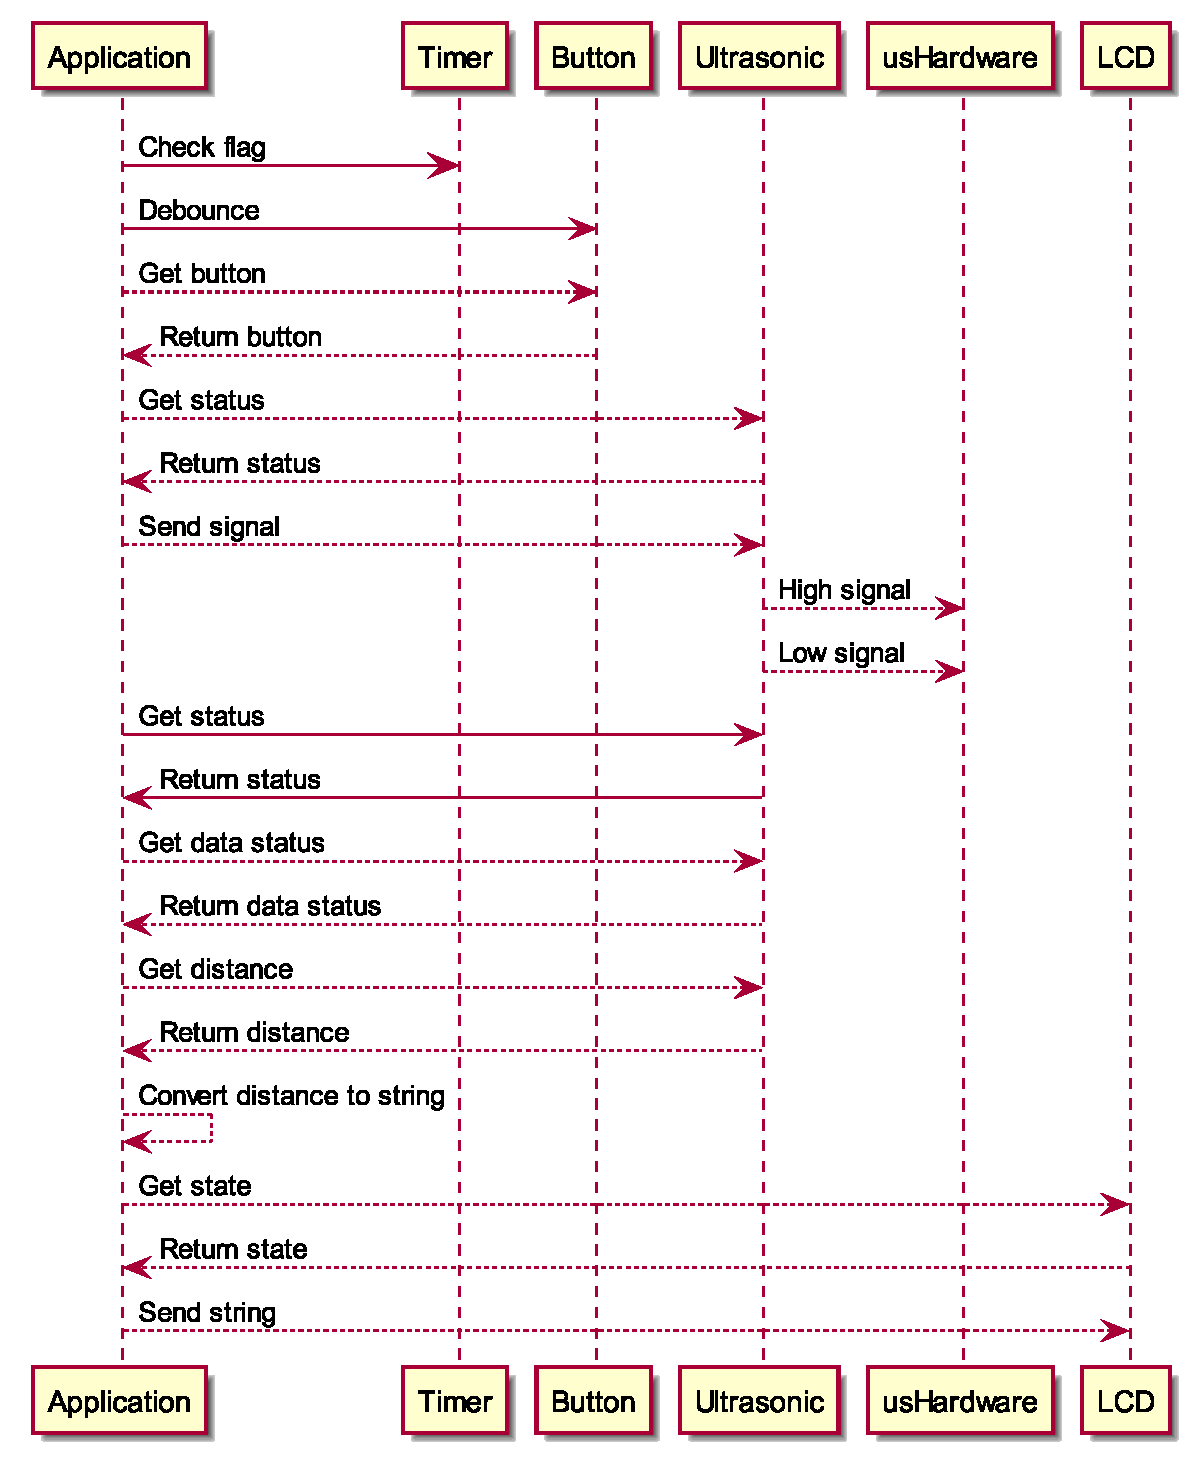
\includegraphics[width=\textwidth,height=\textheight/2,keepaspectratio=true]{inline_umlgraph_2}}
\end{DoxyImageNoCaption}
 Include dependency graph for application.\+c\+:
\nopagebreak
\begin{figure}[H]
\begin{center}
\leavevmode
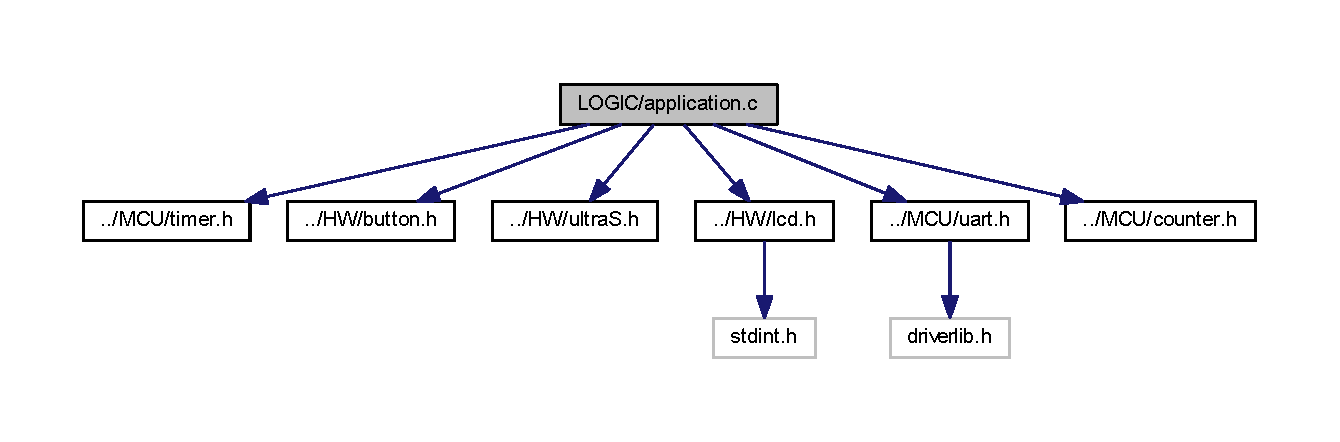
\includegraphics[width=350pt]{application_8c__incl}
\end{center}
\end{figure}
\subsection*{Macros}
\begin{DoxyCompactItemize}
\item 
\#define \hyperlink{application_8c_a62249e384b997229a3e2ae74ade334e2}{D\+E\+L\+AY}~10000U
\end{DoxyCompactItemize}
\subsection*{Functions}
\begin{DoxyCompactItemize}
\item 
void \hyperlink{application_8c_a9dff310201803ed56106c927a9ced9cd}{convert\+U\+Dec} (unsigned long n)
\item 
void \hyperlink{application_8c_aca9e2d049a005223eab8810cc5443efb}{application\+\_\+cyclic} ()
\end{DoxyCompactItemize}
\subsection*{Variables}
\begin{DoxyCompactItemize}
\item 
unsigned long int \hyperlink{application_8c_a74c36f72b6828fd5e43189b2c52f7828}{distance}
\item 
char \hyperlink{application_8c_a9678f24f03848defae48d7a9568ddcb4}{String} \mbox{[}16\mbox{]} = \char`\"{}Kaugus \+: \char`\"{}
\item 
char \hyperlink{application_8c_a6b6430d8f5edc9acef65aa3f3ebfaa51}{String\+Error} \mbox{[}16\mbox{]} = \char`\"{}Error! \char`\"{}
\end{DoxyCompactItemize}


\subsection{Macro Definition Documentation}
\hypertarget{application_8c_a62249e384b997229a3e2ae74ade334e2}{}\label{application_8c_a62249e384b997229a3e2ae74ade334e2} 
\index{application.\+c@{application.\+c}!D\+E\+L\+AY@{D\+E\+L\+AY}}
\index{D\+E\+L\+AY@{D\+E\+L\+AY}!application.\+c@{application.\+c}}
\subsubsection{\texorpdfstring{D\+E\+L\+AY}{DELAY}}
{\footnotesize\ttfamily \#define D\+E\+L\+AY~10000U}

0.\+000625 second delay 

\subsection{Function Documentation}
\hypertarget{application_8c_aca9e2d049a005223eab8810cc5443efb}{}\label{application_8c_aca9e2d049a005223eab8810cc5443efb} 
\index{application.\+c@{application.\+c}!application\+\_\+cyclic@{application\+\_\+cyclic}}
\index{application\+\_\+cyclic@{application\+\_\+cyclic}!application.\+c@{application.\+c}}
\subsubsection{\texorpdfstring{application\+\_\+cyclic()}{application\_cyclic()}}
{\footnotesize\ttfamily void application\+\_\+cyclic (\begin{DoxyParamCaption}{ }\end{DoxyParamCaption})}

The main cyclic function to control the workflow.

Initiates check on button. ~\newline
 If the button has been debounced starts the work (if not already in progress.) ~\newline
 Clears the display and checks with ultrasonic module. ~\newline
 Sends a string to the L\+CD module to be displayed based on value from the ultrasonic module. Here is the call graph for this function\+:
\nopagebreak
\begin{figure}[H]
\begin{center}
\leavevmode
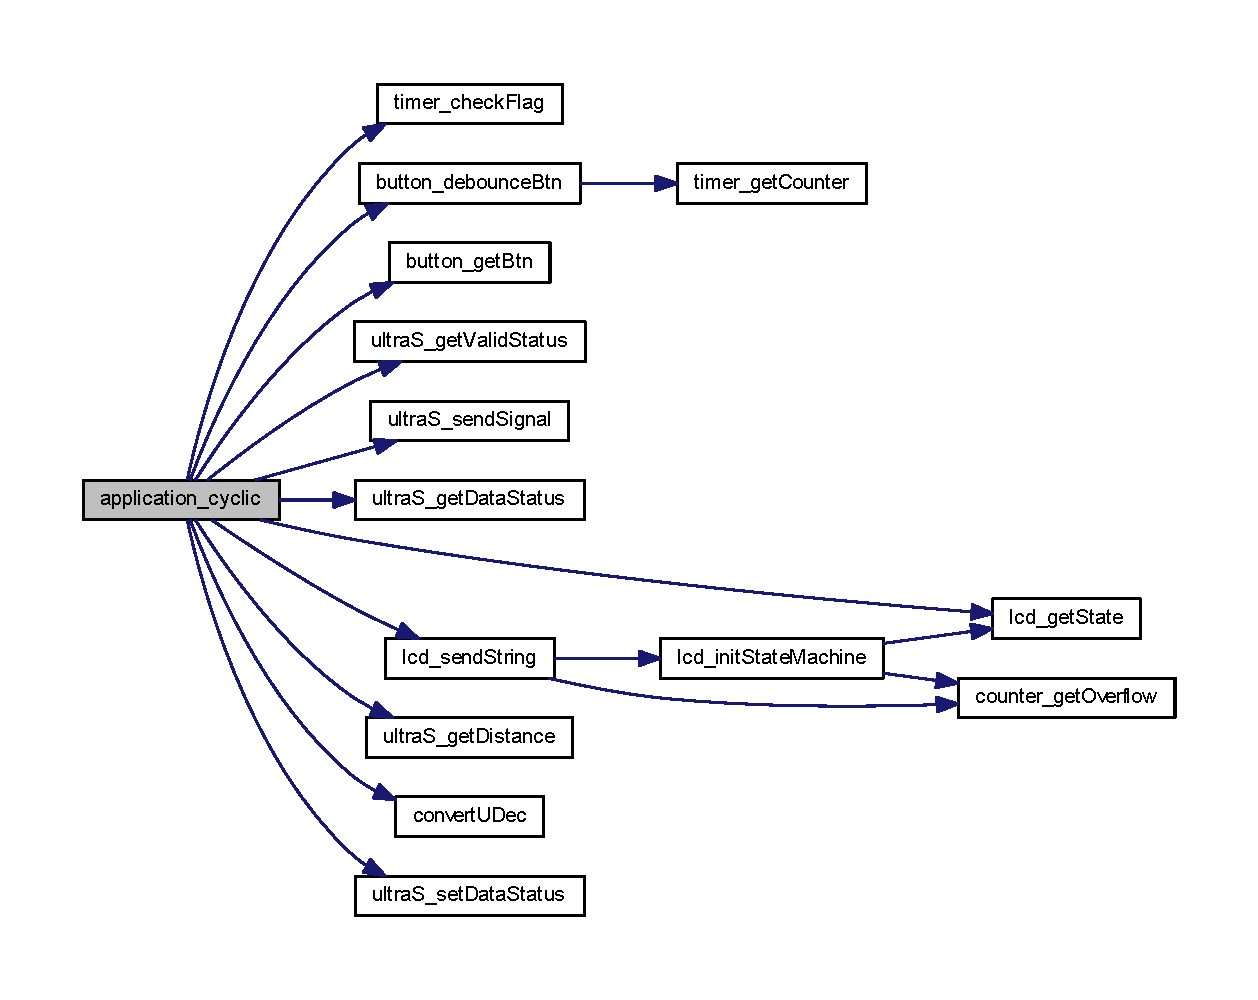
\includegraphics[width=350pt]{application_8c_aca9e2d049a005223eab8810cc5443efb_cgraph}
\end{center}
\end{figure}
\hypertarget{application_8c_a9dff310201803ed56106c927a9ced9cd}{}\label{application_8c_a9dff310201803ed56106c927a9ced9cd} 
\index{application.\+c@{application.\+c}!convert\+U\+Dec@{convert\+U\+Dec}}
\index{convert\+U\+Dec@{convert\+U\+Dec}!application.\+c@{application.\+c}}
\subsubsection{\texorpdfstring{convert\+U\+Dec()}{convertUDec()}}
{\footnotesize\ttfamily void convert\+U\+Dec (\begin{DoxyParamCaption}\item[{unsigned long}]{n }\end{DoxyParamCaption})}

Converts integer value to string

Converts integer to string and places it in {\bfseries String} to the appropriate position ~\newline
 Converts each digit of the value on its own by taking modulo 10 of it and adding a value of 30 to it. ~\newline
 Based on the ascii table where numbers are from 30 to 39.

\begin{DoxyAttention}{Attention}
Currently limited to 4 digit numbers. 
\end{DoxyAttention}

\begin{DoxyParams}{Parameters}
{\em n} & Numeric value to be converted to string. \\
\hline
\end{DoxyParams}
Here is the caller graph for this function\+:
\nopagebreak
\begin{figure}[H]
\begin{center}
\leavevmode
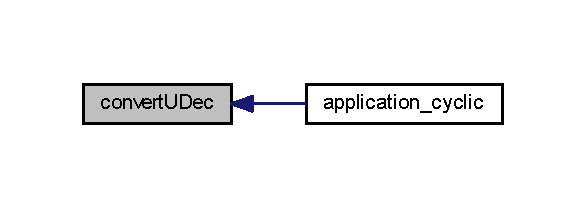
\includegraphics[width=281pt]{application_8c_a9dff310201803ed56106c927a9ced9cd_icgraph}
\end{center}
\end{figure}


\subsection{Variable Documentation}
\hypertarget{application_8c_a74c36f72b6828fd5e43189b2c52f7828}{}\label{application_8c_a74c36f72b6828fd5e43189b2c52f7828} 
\index{application.\+c@{application.\+c}!distance@{distance}}
\index{distance@{distance}!application.\+c@{application.\+c}}
\subsubsection{\texorpdfstring{distance}{distance}}
{\footnotesize\ttfamily unsigned long int distance}

Local variable of distance to be converted to string \hypertarget{application_8c_a9678f24f03848defae48d7a9568ddcb4}{}\label{application_8c_a9678f24f03848defae48d7a9568ddcb4} 
\index{application.\+c@{application.\+c}!String@{String}}
\index{String@{String}!application.\+c@{application.\+c}}
\subsubsection{\texorpdfstring{String}{String}}
{\footnotesize\ttfamily char String\mbox{[}16\mbox{]} = \char`\"{}Kaugus \+: \char`\"{}}

String to be displayed on the L\+CD {\bfseries after} the distance has been added to it \hypertarget{application_8c_a6b6430d8f5edc9acef65aa3f3ebfaa51}{}\label{application_8c_a6b6430d8f5edc9acef65aa3f3ebfaa51} 
\index{application.\+c@{application.\+c}!String\+Error@{String\+Error}}
\index{String\+Error@{String\+Error}!application.\+c@{application.\+c}}
\subsubsection{\texorpdfstring{String\+Error}{StringError}}
{\footnotesize\ttfamily char String\+Error\mbox{[}16\mbox{]} = \char`\"{}Error! \char`\"{}}

String to be displayed on the L\+CD {\bfseries if} the distance fell out of the measurable range 
\hypertarget{counter_8c}{}\section{S\+R\+C/\+M\+C\+U/counter.c File Reference}
\label{counter_8c}\index{S\+R\+C/\+M\+C\+U/counter.\+c@{S\+R\+C/\+M\+C\+U/counter.\+c}}


Documentation for the counter module.  


{\ttfamily \#include $<$driverlib.\+h$>$}\newline
{\ttfamily \#include \char`\"{}counter.\+h\char`\"{}}\newline
\subsection*{Macros}
\begin{DoxyCompactItemize}
\item 
\#define \hyperlink{counter_8c_a1bc63400ff91806a4c1a79caefead705}{T\+I\+M\+E\+TO}~0x\+F\+D\+E8
\end{DoxyCompactItemize}
\subsection*{Functions}
\begin{DoxyCompactItemize}
\item 
unsigned long long int \hyperlink{counter_8c_a71d01976549f4cd7e7ee980186cbe4cb}{counter\+\_\+get\+Overflow} (void)
\item 
void \hyperlink{counter_8c_aba214904e1b489fd2c9a8d6fd85b4756}{counter\+\_\+init} (void)
\item 
\+\_\+\+\_\+interrupt void \hyperlink{counter_8c_aa65b39e29d27a10bf91108fff1f8e852}{counter\+\_\+add\+To\+Timer} (void)
\end{DoxyCompactItemize}
\subsection*{Variables}
\begin{DoxyCompactItemize}
\item 
unsigned long long int \hyperlink{counter_8c_a75e2a4049f11db7e514573608bebadf9}{timer\+B\+\_\+overflow}
\end{DoxyCompactItemize}


\subsection{Detailed Description}
Documentation for the counter module. 

Describes the workings of the counter module. Free running timer for ultrasonic module interrupt. 

\subsection{Macro Definition Documentation}
\hypertarget{counter_8c_a1bc63400ff91806a4c1a79caefead705}{}\label{counter_8c_a1bc63400ff91806a4c1a79caefead705} 
\index{counter.\+c@{counter.\+c}!T\+I\+M\+E\+TO@{T\+I\+M\+E\+TO}}
\index{T\+I\+M\+E\+TO@{T\+I\+M\+E\+TO}!counter.\+c@{counter.\+c}}
\subsubsection{\texorpdfstring{T\+I\+M\+E\+TO}{TIMETO}}
{\footnotesize\ttfamily \#define T\+I\+M\+E\+TO~0x\+F\+D\+E8}

32.\+5 ms cycle for timer A. Calculated with 16\+M\+Hz S\+M\+C\+LK with divider 16 

\subsection{Function Documentation}
\hypertarget{counter_8c_aa65b39e29d27a10bf91108fff1f8e852}{}\label{counter_8c_aa65b39e29d27a10bf91108fff1f8e852} 
\index{counter.\+c@{counter.\+c}!counter\+\_\+add\+To\+Timer@{counter\+\_\+add\+To\+Timer}}
\index{counter\+\_\+add\+To\+Timer@{counter\+\_\+add\+To\+Timer}!counter.\+c@{counter.\+c}}
\subsubsection{\texorpdfstring{counter\+\_\+add\+To\+Timer()}{counter\_addToTimer()}}
{\footnotesize\ttfamily \+\_\+\+\_\+interrupt void counter\+\_\+add\+To\+Timer (\begin{DoxyParamCaption}\item[{void}]{ }\end{DoxyParamCaption})}

Interrupt vector for timer\+B0.

Is triggered when the timerB\textquotesingle{}s value reaches T\+I\+M\+E\+TO and resets back to 0. \hypertarget{counter_8c_a71d01976549f4cd7e7ee980186cbe4cb}{}\label{counter_8c_a71d01976549f4cd7e7ee980186cbe4cb} 
\index{counter.\+c@{counter.\+c}!counter\+\_\+get\+Overflow@{counter\+\_\+get\+Overflow}}
\index{counter\+\_\+get\+Overflow@{counter\+\_\+get\+Overflow}!counter.\+c@{counter.\+c}}
\subsubsection{\texorpdfstring{counter\+\_\+get\+Overflow()}{counter\_getOverflow()}}
{\footnotesize\ttfamily unsigned long long int counter\+\_\+get\+Overflow (\begin{DoxyParamCaption}\item[{void}]{ }\end{DoxyParamCaption})}

Get timerA\textquotesingle{}s interrupt\+Counter.

\begin{DoxyReturn}{Returns}
timer\+B\+\_\+overflow 
\end{DoxyReturn}
\hypertarget{counter_8c_aba214904e1b489fd2c9a8d6fd85b4756}{}\label{counter_8c_aba214904e1b489fd2c9a8d6fd85b4756} 
\index{counter.\+c@{counter.\+c}!counter\+\_\+init@{counter\+\_\+init}}
\index{counter\+\_\+init@{counter\+\_\+init}!counter.\+c@{counter.\+c}}
\subsubsection{\texorpdfstring{counter\+\_\+init()}{counter\_init()}}
{\footnotesize\ttfamily void counter\+\_\+init (\begin{DoxyParamCaption}\item[{void}]{ }\end{DoxyParamCaption})}

Initializes Timer B in up mode with T\+I\+M\+E\+TO ms cycle time. 

\subsection{Variable Documentation}
\hypertarget{counter_8c_a75e2a4049f11db7e514573608bebadf9}{}\label{counter_8c_a75e2a4049f11db7e514573608bebadf9} 
\index{counter.\+c@{counter.\+c}!timer\+B\+\_\+overflow@{timer\+B\+\_\+overflow}}
\index{timer\+B\+\_\+overflow@{timer\+B\+\_\+overflow}!counter.\+c@{counter.\+c}}
\subsubsection{\texorpdfstring{timer\+B\+\_\+overflow}{timerB\_overflow}}
{\footnotesize\ttfamily unsigned long long int timer\+B\+\_\+overflow}

Maximum time; Will only result in false data when it overflow itself. $\sim$4 years 
\hypertarget{counter_8h}{}\section{M\+C\+U/counter.h File Reference}
\label{counter_8h}\index{M\+C\+U/counter.\+h@{M\+C\+U/counter.\+h}}


\subsection{Detailed Description}
Documentation for the counter module\textquotesingle{}s header. 

Global macro defines. This graph shows which files directly or indirectly include this file\+:\nopagebreak
\begin{figure}[H]
\begin{center}
\leavevmode
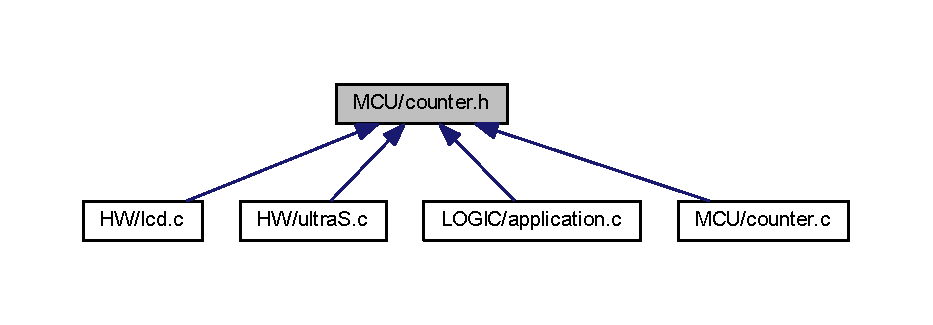
\includegraphics[width=350pt]{counter_8h__dep__incl}
\end{center}
\end{figure}
\subsection*{Macros}
\begin{DoxyCompactItemize}
\item 
\#define \hyperlink{counter_8h_a383bc9817a0a055d07f3b2b948fb0b7e}{counter\+\_\+en\+T\+BI}(timer\+Base)~Timer\+\_\+\+B\+\_\+enable\+Interrupt(timer\+Base)			/$\ast$ Enable interrupts by Timer B $\ast$/
\begin{DoxyCompactList}\small\item\em Sets local gpio to appropriate board function of similar name. \end{DoxyCompactList}\item 
\#define \hyperlink{counter_8h_ad53f7cf4741c618c5cce65f273bd52c9}{counter\+\_\+di\+T\+BI}(timer\+Base)~Timer\+\_\+\+B\+\_\+disable\+Interrupt(timer\+Base)			/$\ast$ Disable interrupts by Timer B $\ast$/
\begin{DoxyCompactList}\small\item\em Sets local gpio to appropriate board function of similar name. \end{DoxyCompactList}\item 
\#define \hyperlink{counter_8h_abffd74faf0296b433da654c54555bf91}{counter\+\_\+get\+Count\+Value}(timer\+Base)~Timer\+\_\+\+B\+\_\+get\+Counter\+Value(timer\+Base);
\begin{DoxyCompactList}\small\item\em Sets local gpio to appropriate board function of similar name. \end{DoxyCompactList}\item 
\#define \hyperlink{counter_8h_a987db31c103beded52c16d4553224150}{counter\+\_\+timer\+Base}~T\+I\+M\+E\+R\+\_\+\+B0\+\_\+\+B\+A\+SE
\end{DoxyCompactItemize}


\subsection{Macro Definition Documentation}
\hypertarget{counter_8h_ad53f7cf4741c618c5cce65f273bd52c9}{}\label{counter_8h_ad53f7cf4741c618c5cce65f273bd52c9} 
\index{counter.\+h@{counter.\+h}!counter\+\_\+di\+T\+BI@{counter\+\_\+di\+T\+BI}}
\index{counter\+\_\+di\+T\+BI@{counter\+\_\+di\+T\+BI}!counter.\+h@{counter.\+h}}
\subsubsection{\texorpdfstring{counter\+\_\+di\+T\+BI}{counter\_diTBI}}
{\footnotesize\ttfamily \#define counter\+\_\+di\+T\+BI(\begin{DoxyParamCaption}\item[{}]{timer\+Base }\end{DoxyParamCaption})~Timer\+\_\+\+B\+\_\+disable\+Interrupt(timer\+Base)			/$\ast$ Disable interrupts by Timer B $\ast$/}



Sets local gpio to appropriate board function of similar name. 

Disables interrupts by {\bfseries timer\+Base} timer. \hypertarget{counter_8h_a383bc9817a0a055d07f3b2b948fb0b7e}{}\label{counter_8h_a383bc9817a0a055d07f3b2b948fb0b7e} 
\index{counter.\+h@{counter.\+h}!counter\+\_\+en\+T\+BI@{counter\+\_\+en\+T\+BI}}
\index{counter\+\_\+en\+T\+BI@{counter\+\_\+en\+T\+BI}!counter.\+h@{counter.\+h}}
\subsubsection{\texorpdfstring{counter\+\_\+en\+T\+BI}{counter\_enTBI}}
{\footnotesize\ttfamily \#define counter\+\_\+en\+T\+BI(\begin{DoxyParamCaption}\item[{}]{timer\+Base }\end{DoxyParamCaption})~Timer\+\_\+\+B\+\_\+enable\+Interrupt(timer\+Base)			/$\ast$ Enable interrupts by Timer B $\ast$/}



Sets local gpio to appropriate board function of similar name. 

Enables interrupts by {\bfseries timer\+Base} timer. \hypertarget{counter_8h_abffd74faf0296b433da654c54555bf91}{}\label{counter_8h_abffd74faf0296b433da654c54555bf91} 
\index{counter.\+h@{counter.\+h}!counter\+\_\+get\+Count\+Value@{counter\+\_\+get\+Count\+Value}}
\index{counter\+\_\+get\+Count\+Value@{counter\+\_\+get\+Count\+Value}!counter.\+h@{counter.\+h}}
\subsubsection{\texorpdfstring{counter\+\_\+get\+Count\+Value}{counter\_getCountValue}}
{\footnotesize\ttfamily \#define counter\+\_\+get\+Count\+Value(\begin{DoxyParamCaption}\item[{}]{timer\+Base }\end{DoxyParamCaption})~Timer\+\_\+\+B\+\_\+get\+Counter\+Value(timer\+Base);}



Sets local gpio to appropriate board function of similar name. 

Gets the current timer value form {\bfseries timer\+Base} timer. \hypertarget{counter_8h_a987db31c103beded52c16d4553224150}{}\label{counter_8h_a987db31c103beded52c16d4553224150} 
\index{counter.\+h@{counter.\+h}!counter\+\_\+timer\+Base@{counter\+\_\+timer\+Base}}
\index{counter\+\_\+timer\+Base@{counter\+\_\+timer\+Base}!counter.\+h@{counter.\+h}}
\subsubsection{\texorpdfstring{counter\+\_\+timer\+Base}{counter\_timerBase}}
{\footnotesize\ttfamily \#define counter\+\_\+timer\+Base~T\+I\+M\+E\+R\+\_\+\+B0\+\_\+\+B\+A\+SE}

The used timer\textquotesingle{}s timer\+Base for the counter module 
\hypertarget{timer_8c}{}\section{M\+C\+U/timer.c File Reference}
\label{timer_8c}\index{M\+C\+U/timer.\+c@{M\+C\+U/timer.\+c}}


\subsection{Detailed Description}
Documentation for the timer module. 

Describes the workings of the timer module. Is used to debounce a button press. Include dependency graph for timer.\+c\+:\nopagebreak
\begin{figure}[H]
\begin{center}
\leavevmode
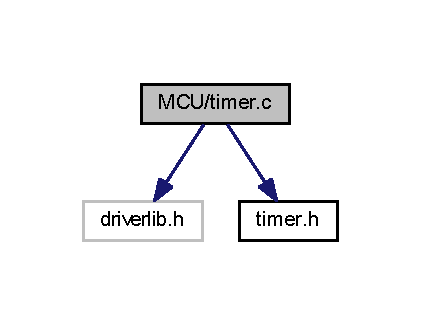
\includegraphics[width=202pt]{timer_8c__incl}
\end{center}
\end{figure}
\subsection*{Macros}
\begin{DoxyCompactItemize}
\item 
\#define \hyperlink{timer_8c_a1bc63400ff91806a4c1a79caefead705}{T\+I\+M\+E\+TO}~0x1\+F40
\end{DoxyCompactItemize}
\subsection*{Functions}
\begin{DoxyCompactItemize}
\item 
void \hyperlink{timer_8c_a7b8ab79df77b57475a5494f5f81c3bd9}{timer\+\_\+init} (void)
\item 
void \hyperlink{timer_8c_a50eeb50a751ec06e0d58643f45c92874}{timer\+\_\+check\+Flag} ()
\item 
int \hyperlink{timer_8c_a1021e8241d2431ad3c33e4dca3479e30}{timer\+\_\+get\+Counter} (void)
\item 
\+\_\+\+\_\+interrupt void \hyperlink{timer_8c_a5c04b6546e82f2e5f0af1410addf382c}{timer\+\_\+debouncing\+Btn} (void)
\end{DoxyCompactItemize}
\subsection*{Variables}
\begin{DoxyCompactItemize}
\item 
unsigned long long int \hyperlink{timer_8c_a34a34f6517460d2f8fff3dbfc8764ac0}{interrupt\+Counter}
\item 
short \hyperlink{timer_8c_a0939402298c3765d4bbc62cea55ea0be}{timer\+Flag} = 0
\end{DoxyCompactItemize}


\subsection{Macro Definition Documentation}
\hypertarget{timer_8c_a1bc63400ff91806a4c1a79caefead705}{}\label{timer_8c_a1bc63400ff91806a4c1a79caefead705} 
\index{timer.\+c@{timer.\+c}!T\+I\+M\+E\+TO@{T\+I\+M\+E\+TO}}
\index{T\+I\+M\+E\+TO@{T\+I\+M\+E\+TO}!timer.\+c@{timer.\+c}}
\subsubsection{\texorpdfstring{T\+I\+M\+E\+TO}{TIMETO}}
{\footnotesize\ttfamily \#define T\+I\+M\+E\+TO~0x1\+F40}

0.\+5 ms cycle for timer A. Calculated with 16\+M\+Hz S\+M\+C\+LK with divider 1 

\subsection{Function Documentation}
\hypertarget{timer_8c_a50eeb50a751ec06e0d58643f45c92874}{}\label{timer_8c_a50eeb50a751ec06e0d58643f45c92874} 
\index{timer.\+c@{timer.\+c}!timer\+\_\+check\+Flag@{timer\+\_\+check\+Flag}}
\index{timer\+\_\+check\+Flag@{timer\+\_\+check\+Flag}!timer.\+c@{timer.\+c}}
\subsubsection{\texorpdfstring{timer\+\_\+check\+Flag()}{timer\_checkFlag()}}
{\footnotesize\ttfamily void timer\+\_\+check\+Flag (\begin{DoxyParamCaption}{ }\end{DoxyParamCaption})}

Checks whether there has been a timer interrupt and increments a counter if so.

Is called from application level in every cycle. timer\+Flag is set to true whenever a timer A interrupt has occurred. Is used to get a delay of T\+I\+M\+E\+TO $\ast$ interrupt\+Counter. Here is the caller graph for this function\+:\nopagebreak
\begin{figure}[H]
\begin{center}
\leavevmode
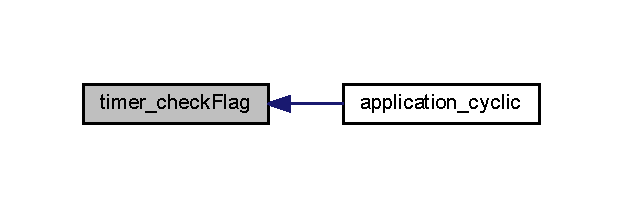
\includegraphics[width=299pt]{timer_8c_a50eeb50a751ec06e0d58643f45c92874_icgraph}
\end{center}
\end{figure}
\hypertarget{timer_8c_a5c04b6546e82f2e5f0af1410addf382c}{}\label{timer_8c_a5c04b6546e82f2e5f0af1410addf382c} 
\index{timer.\+c@{timer.\+c}!timer\+\_\+debouncing\+Btn@{timer\+\_\+debouncing\+Btn}}
\index{timer\+\_\+debouncing\+Btn@{timer\+\_\+debouncing\+Btn}!timer.\+c@{timer.\+c}}
\subsubsection{\texorpdfstring{timer\+\_\+debouncing\+Btn()}{timer\_debouncingBtn()}}
{\footnotesize\ttfamily \+\_\+\+\_\+interrupt void timer\+\_\+debouncing\+Btn (\begin{DoxyParamCaption}\item[{void}]{ }\end{DoxyParamCaption})}

Interrupt vector for timer\+A0.

Is triggered when the timerA\textquotesingle{}s value reaches T\+I\+M\+E\+TO and resets back to 0. \hypertarget{timer_8c_a1021e8241d2431ad3c33e4dca3479e30}{}\label{timer_8c_a1021e8241d2431ad3c33e4dca3479e30} 
\index{timer.\+c@{timer.\+c}!timer\+\_\+get\+Counter@{timer\+\_\+get\+Counter}}
\index{timer\+\_\+get\+Counter@{timer\+\_\+get\+Counter}!timer.\+c@{timer.\+c}}
\subsubsection{\texorpdfstring{timer\+\_\+get\+Counter()}{timer\_getCounter()}}
{\footnotesize\ttfamily int timer\+\_\+get\+Counter (\begin{DoxyParamCaption}\item[{void}]{ }\end{DoxyParamCaption})}

Get timerA\textquotesingle{}s interrupt\+Counter.

\begin{DoxyReturn}{Returns}
interrupt\+Counter 
\end{DoxyReturn}
Here is the caller graph for this function\+:\nopagebreak
\begin{figure}[H]
\begin{center}
\leavevmode
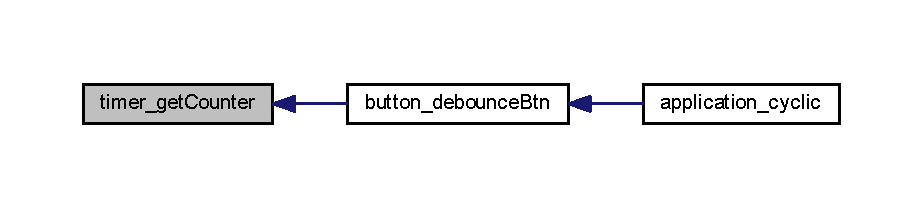
\includegraphics[width=350pt]{timer_8c_a1021e8241d2431ad3c33e4dca3479e30_icgraph}
\end{center}
\end{figure}
\hypertarget{timer_8c_a7b8ab79df77b57475a5494f5f81c3bd9}{}\label{timer_8c_a7b8ab79df77b57475a5494f5f81c3bd9} 
\index{timer.\+c@{timer.\+c}!timer\+\_\+init@{timer\+\_\+init}}
\index{timer\+\_\+init@{timer\+\_\+init}!timer.\+c@{timer.\+c}}
\subsubsection{\texorpdfstring{timer\+\_\+init()}{timer\_init()}}
{\footnotesize\ttfamily void timer\+\_\+init (\begin{DoxyParamCaption}\item[{void}]{ }\end{DoxyParamCaption})}

Initializes Timer A in up mode with T\+I\+M\+E\+TO ms cycle time. 

\subsection{Variable Documentation}
\hypertarget{timer_8c_a34a34f6517460d2f8fff3dbfc8764ac0}{}\label{timer_8c_a34a34f6517460d2f8fff3dbfc8764ac0} 
\index{timer.\+c@{timer.\+c}!interrupt\+Counter@{interrupt\+Counter}}
\index{interrupt\+Counter@{interrupt\+Counter}!timer.\+c@{timer.\+c}}
\subsubsection{\texorpdfstring{interrupt\+Counter}{interruptCounter}}
{\footnotesize\ttfamily unsigned long long int interrupt\+Counter}

Times the timer A interrupt has to taken place \hypertarget{timer_8c_a0939402298c3765d4bbc62cea55ea0be}{}\label{timer_8c_a0939402298c3765d4bbc62cea55ea0be} 
\index{timer.\+c@{timer.\+c}!timer\+Flag@{timer\+Flag}}
\index{timer\+Flag@{timer\+Flag}!timer.\+c@{timer.\+c}}
\subsubsection{\texorpdfstring{timer\+Flag}{timerFlag}}
{\footnotesize\ttfamily short timer\+Flag = 0}

Flag to check whether an interrupt has occured or not. 
\hypertarget{timer_8h}{}\section{M\+C\+U/timer.h File Reference}
\label{timer_8h}\index{M\+C\+U/timer.\+h@{M\+C\+U/timer.\+h}}


\subsection{Detailed Description}
Documentation for the timer module\textquotesingle{}s header. 

Global macro defines. This graph shows which files directly or indirectly include this file\+:\nopagebreak
\begin{figure}[H]
\begin{center}
\leavevmode
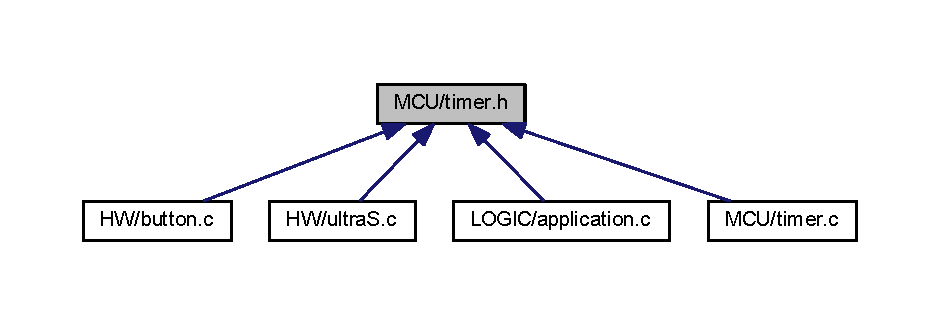
\includegraphics[width=350pt]{timer_8h__dep__incl}
\end{center}
\end{figure}
\subsection*{Macros}
\begin{DoxyCompactItemize}
\item 
\#define \hyperlink{timer_8h_a0318b2b589fd22bb3f79963235687bab}{timer\+\_\+en\+T\+AI}(timer\+Base)~Timer\+\_\+\+A\+\_\+enable\+Interrupt(timer\+Base)
\begin{DoxyCompactList}\small\item\em Sets local gpio to appropriate board function of similar name. \end{DoxyCompactList}\item 
\#define \hyperlink{timer_8h_a2ffba2fe10bb1cf8926bbff35cb1df77}{timer\+\_\+di\+T\+AI}(timer\+Base)~Timer\+\_\+\+A\+\_\+disable\+Interrupt(timer\+Base)
\begin{DoxyCompactList}\small\item\em Sets local gpio to appropriate board function of similar name. \end{DoxyCompactList}\item 
\#define \hyperlink{timer_8h_a65b751ef29ef9e38c2aa875ef7df1fa5}{timer\+\_\+timer\+Base}~T\+I\+M\+E\+R\+\_\+\+A0\+\_\+\+B\+A\+SE
\end{DoxyCompactItemize}


\subsection{Macro Definition Documentation}
\hypertarget{timer_8h_a2ffba2fe10bb1cf8926bbff35cb1df77}{}\label{timer_8h_a2ffba2fe10bb1cf8926bbff35cb1df77} 
\index{timer.\+h@{timer.\+h}!timer\+\_\+di\+T\+AI@{timer\+\_\+di\+T\+AI}}
\index{timer\+\_\+di\+T\+AI@{timer\+\_\+di\+T\+AI}!timer.\+h@{timer.\+h}}
\subsubsection{\texorpdfstring{timer\+\_\+di\+T\+AI}{timer\_diTAI}}
{\footnotesize\ttfamily \#define timer\+\_\+di\+T\+AI(\begin{DoxyParamCaption}\item[{}]{timer\+Base }\end{DoxyParamCaption})~Timer\+\_\+\+A\+\_\+disable\+Interrupt(timer\+Base)}



Sets local gpio to appropriate board function of similar name. 

Disables interrupts by {\bfseries timer\+Base} timer. \hypertarget{timer_8h_a0318b2b589fd22bb3f79963235687bab}{}\label{timer_8h_a0318b2b589fd22bb3f79963235687bab} 
\index{timer.\+h@{timer.\+h}!timer\+\_\+en\+T\+AI@{timer\+\_\+en\+T\+AI}}
\index{timer\+\_\+en\+T\+AI@{timer\+\_\+en\+T\+AI}!timer.\+h@{timer.\+h}}
\subsubsection{\texorpdfstring{timer\+\_\+en\+T\+AI}{timer\_enTAI}}
{\footnotesize\ttfamily \#define timer\+\_\+en\+T\+AI(\begin{DoxyParamCaption}\item[{}]{timer\+Base }\end{DoxyParamCaption})~Timer\+\_\+\+A\+\_\+enable\+Interrupt(timer\+Base)}



Sets local gpio to appropriate board function of similar name. 

Enables interrupts by {\bfseries timer\+Base} timer. \hypertarget{timer_8h_a65b751ef29ef9e38c2aa875ef7df1fa5}{}\label{timer_8h_a65b751ef29ef9e38c2aa875ef7df1fa5} 
\index{timer.\+h@{timer.\+h}!timer\+\_\+timer\+Base@{timer\+\_\+timer\+Base}}
\index{timer\+\_\+timer\+Base@{timer\+\_\+timer\+Base}!timer.\+h@{timer.\+h}}
\subsubsection{\texorpdfstring{timer\+\_\+timer\+Base}{timer\_timerBase}}
{\footnotesize\ttfamily \#define timer\+\_\+timer\+Base~T\+I\+M\+E\+R\+\_\+\+A0\+\_\+\+B\+A\+SE}

The used timer\textquotesingle{}s timer\+Base for the timer module 
%--- End generated contents ---

% Index
\backmatter
\newpage
\phantomsection
\clearemptydoublepage
\addcontentsline{toc}{chapter}{Index}
\printindex

\end{document}
